
%% Add the 'procedia' option to approximate to the Word template
\documentclass[3p,procedia]{elsarticle}
\usepackage{ecrc}
\usepackage{color,soul}
\usepackage{multirow}
\usepackage{booktabs}
\graphicspath{{images/}}
\usepackage{lscape}
\usepackage{amssymb}
\usepackage{lineno}
\usepackage{hyperref}
\usepackage{subfig}
\usepackage[export]{adjustbox}
\usepackage{diagbox}

\volume{00}
\firstpage{1}
%\journalname{Forest ecology and management}
\runauth{Gilles A. et al.}

\DeclareUnicodeCharacter{00E4}{\"a}% pour -niittyla

\begin{document}

\begin{frontmatter}

\author[label1]{Gilles Arthur}
\ead{arthur.gilles@uliege.be}
\author[label1]{Lisein Jonathan}
\author[label2]{Lemaire Jean}
\author[label2]{Cansel Juliette}
\author[label3]{Piedallu Christian}
\author[label1]{Claessens Hugues}

\fntext[label1]{Liège University - Faculty of Gembloux Agro-Bio Tech - unit of forest ressources managment}
\fntext[label2]{Centre National de la propriété forestière}
\fntext[label3]{Université de Lorraine, AgroParisTech, Inra, Silva, F-54000 Nancy, AgroParisTech, 14 rue Girardet, F-54042 Nancy Cedex, France}


\dochead{Original research papers}

\title{Spruce vulnerability to bark beetle attack vary with altitude and topographic position: a remote sensing analysis in Belgium and France}
\begin{abstract}
	
\iffalse
Following the droughts of 2018 to 2020, numerous Norway spruce diebacks were caused by bark beetles 
%(Ips typographus/ Pityogenes chalcographus)
outbreaks in Wallonia and in the Grand-Est. 
A methodology for detection the health status of spruce was developed based on satellite imagery from the European Union's Earth Observation Programme.
The time series of satellite images allowed the modelling of the spectral response of healthy spruce forests over the seasons. Deviations from this seasonal vegetation index trajectory for a healthy spruce stand are caused by a decrease in photosynthetic activity of the forest canopy.
This decrease in photosynthesis is caused by a bark beetle attack and is detected automatically.
This technique, inspired by the work of INRAe, is robust because of the redundancy of the information from the spatial images, which are repeated every 3-4 weeks. 
The method results in the production of annual maps of the health status of the Walloon and Grand-Est spruce forests.
The most important damage occurred in the years 2018-2019, affecting 2.8\% of the total area of spruce stands in Wallonia.
Although the main part of the crisis seems to be behind us, it remains to draw the necessary conclusions.
The relationship between climatic conditions and the presence of the bark beetle has proven to be complex in Wallonia.
Nevertheless, a very strong relationship between altitude and the presence of bark beetle damage could be demonstrated.
Stands below 300m in altitude were indeed much more affected.
Moreover, forest sites located on steep slopes ( $\ge$  20 \%), whether on cold or warm slopes, are more affected than sites located on low slopes (plateaus).
In the Grand-Est, the peak of the crisis has been reached in 2019-2020. Altitude and slopes are not strongly influencing factors for spruce dieback. 

\fi
\end{abstract}

\begin{keyword}
  Norway spuce \sep Species vulnerability \sep Bark Beetle \sep forest management \sep forest site \sep topographic condition \sep time series \sep Sentinel-2
\end{keyword}

\end{frontmatter}

\linenumbers

\section{Introduction}

Global changes are increasing the risk of disturbances in forest environment: frequency and intensity of abiotic (fire, storm, drough) and biotic (pest invasion) will be more recurrent \citep{lindner_climate_2010}.
In Western Europe, we expect a decrease of precipitation and a increase of drought events during the vegetation period, which will impact the actual geographic distribution of tree species \citep{hanewinkel2013climate}.
Due to the long time required to complete a forest revolutions, forest managers have to anticipate likely changes in climate conditions by modifying the forest tree species they used to regenerate at a particular location, in a way that the future environmental conditions of the forest site still meet the species requirements.
Norway spruce (\textit{Picea abies L. Karst}) is one of the most important economic plant species in Europe \citep{nystedt_norway_2013}.
Its productivity comes with a demanding amount of precipitation, thus making it sensitive to climate changes.
Plus, its major pest is bark beetle that cause important outbreak after storm, which provide breeding material e.g. windfalls and candle, or after severe drougth that weaken trees.
A recent bark beetle crisis, triggered by the exceptionally hot and dry weather of 2018, occurred in Western Europe and lasted until 2021. 
It has urged the need of adapting forest management practices. 
Indeed, forest practitioners have to decide now which species will replace Norway spruce in the thousands of clear-cutted hectares decimated by bark beetle attacks. 
The decision-making of replanting spruce requires a proper understanding of both Norway spruce and bark beetle autecology.

The Norway spruce is adapted to wide range of environmental conditions, although it prefers cold and humid climate.
It is naturally present in part of the Grand-Est (Vosges mountains, France) and artificially in Wallonia (Belgium). In both regions, it was introduced during the second half of the 19th century \citep{Noirfalise_1975,guinier_trois_1959}.
The massive reforestations occurring at this time have led to the formation of large pure even-aged stands.
Moist and reasonably fertile soils are favourable for its productive cultivation \citep{horgan_guide_2003}.
It usually develops a taproot system with fine roots in shallow depth, although the roots go deeper on restrictive soil conditions \citep{puhe_roots_2003}.   
The precipitation are its primary water source \citep{tjoelker_outline_2007} and lack of water induces stress that affect growth and health of the tree. 
The most important pest for Norway spruce are bark beetles species.
The bark beetle species \textit{Ips typographus} causes the most important damages.
Thus in this paper, bark beetle refers to this species.
Stressed Norway spruce produce volatile compounds which attract bark beetles, making himself more susceptible to pest attack \citep{netherer_waterlimiting_2015,netherer_interactions_2021}.
Bark beetle is ubiquitous in the forest and their populations are usually low (endemic phasis).
Many stressed trees  cause a shift to an epidemic phasis with a explosion of bark beetle populations during which even healthy trees are massively attacked \citep{kautz_individual_2014}.
The life cycle of bark beetle depends on temperature and photoperiod \citep{annila_influence_1969, baier_phenipscomprehensive_2007}.
In North Europe, the bark beetle is univoltine (one single generation) but it is multivoltine (breed two or even three generations) in Western and Central Europe \citep{annila_influence_1969}.
After spring swarming, the adult enter in the bark and burrow wood to make brood gallery where they mate and lay the eggs that mature to larvae into the phloem \citep{hlasny_bark_2021}.
The bark beetle adult can re-emerge and swarm a second time to give birth to one sister brood \citep{zolubas_1995}.
After the larvae maturation that last about seven weeks \citep{baier_phenipscomprehensive_2007}, the new generation of beetles emerge and attack the direct surrounding trees \citep{zolubas_1995}.
Attacked trees defend themselves by pulsing resin to kill the bark beetle but these defence failed to resist again numerous simultaneous attacks that induce their decline and rapid death.
The Norway spruce dieback goes through three physiological stages which are denominated green, red and grey stage.
During the green stage, the bark beetle has succeeded to penetrate the phloem and the spruce retains its green needles. 
The tree is still alive but begins to suffer of water shortage caused by sap conduction problem. 
After several weeks, the red stage is reached when the needles turn brown-red. The tree is recently dead and the dry needles start to fall.
When all the needles of the spruce have fallen off and the grey bark of the trunk is visible, the grey stage is reached \citep{abdullah_european_2018}. 
To control the infestation of bark beetle, the practical solutions are limited. 
The use of phytosanitary product is forbidden in Belgian and French forest.
Pheromone trap systems are commercialized to fight bark beetle
 but they failed to limit the economic loss in case of large outbreak \citep{kuhn_pheromone_2022}.
The only solution to decrease the damage cause by outbreak is to remove felled tree before the swarming to take out the ideal breeding material of the forest and to realize sanitary cutting when the tree is attacked by bark beetle at the green stage to decrease the bark beetle population. 


The European Union’s earth observation programme, with its satellite twin constellation Sentinel-2A and Sentinel-2B, provides free earth imagery with a high revisit time, which have been intensively used for forestry purpose. 
Time series of Sentinel-2 (S2) images enable to model the phenology courses of vegetation indices in order to detect forest disturbances \citep{low_phenology_2020}, like the one caused by bark beetle outbreaks.
Infestation maps of the last sanitary crisis have been generated for Germany \citep{ali_canopy_2021,thonfeld_first_2022}, Czech Republic \citep{barta_early_2021}, Italy \citep{dalponte_mapping_2022} and France \citep{nardi_drought_2022}. 
This paper aims at studying the extent and the dynamic of the 2017-2021 bark beetle outbreak in Wallonia and in the Grand-Est.
To this end, we map Norway spruce dieback using S2 time series.
Then, we analyse the relationship between forest stands, bark beetle and environmental conditions in order to determine the most sensitive forest sites where Norway spruce should not be regenerated.


\section{Material and methods}
\subsection{Study area}

The study area was located in Wallonia (south of Belgium) and in the Grand-Est (north-east of France).
The Walloon forest covers 554,600 ha and  Norway spruce stand occupies a quarter of this forest \citep{Alderweireld_2015}. 
%Two thirds of the Walloon spruce forest is located above 400 m altitude. 
The Norway spruce covers seven percent of the 1939,000 ha the Grand-Est forest \citep{IGN2022}. 
%The majority of Norway spruce stand of this region grow between 400m and 900m. 

The both neighbour countries share some similar environmental conditions.
The Grand-Est and Wallonia are included in the temperate oceanic bioclimatic zone \citep{lindner_climate_2010}.

The 24 natural regions of Wallonia and Grand-Est depend of the climate and influence the tree species distribution \citep{walthert_tree_2017}.
Some natural regions have analogous climate and allow presence of the same tree species.
%The Norway spruce of central Europe need a moutain climate.
To better understand the dieback of Norway spruce, the French and Walloon natural regions have been grouped by average temperature and precipitation during the growing season in three homogeneous climatic areas: Ardenne, Plains and Vosges (Figure \ref{fig:clim}).
The Plains is characterized by a temperature between 15.5°C and 18°C and by precipitations between 300 mm and 400 mm.
Natural regions with a temperature between 14°C and 15.5°C and a average precipitation between 400 mm and 450 mm correspond to climatic area of Ardenne.
Vosges are natural regions with temperature varies between 15.5°C and 17 °C and the precipitation between 425 mm and 600 mm.
The Figure \ref{fig:situ} shows localisation of the three climatic areas. 
The climate variables for Wallonia have been provided by the Institut Royal Météorologique and come from the climate map Digitalis \citep{piedallu_presentation_2014} for the Grand-Est.
\begin{figure}[htbp] 
	\centering
	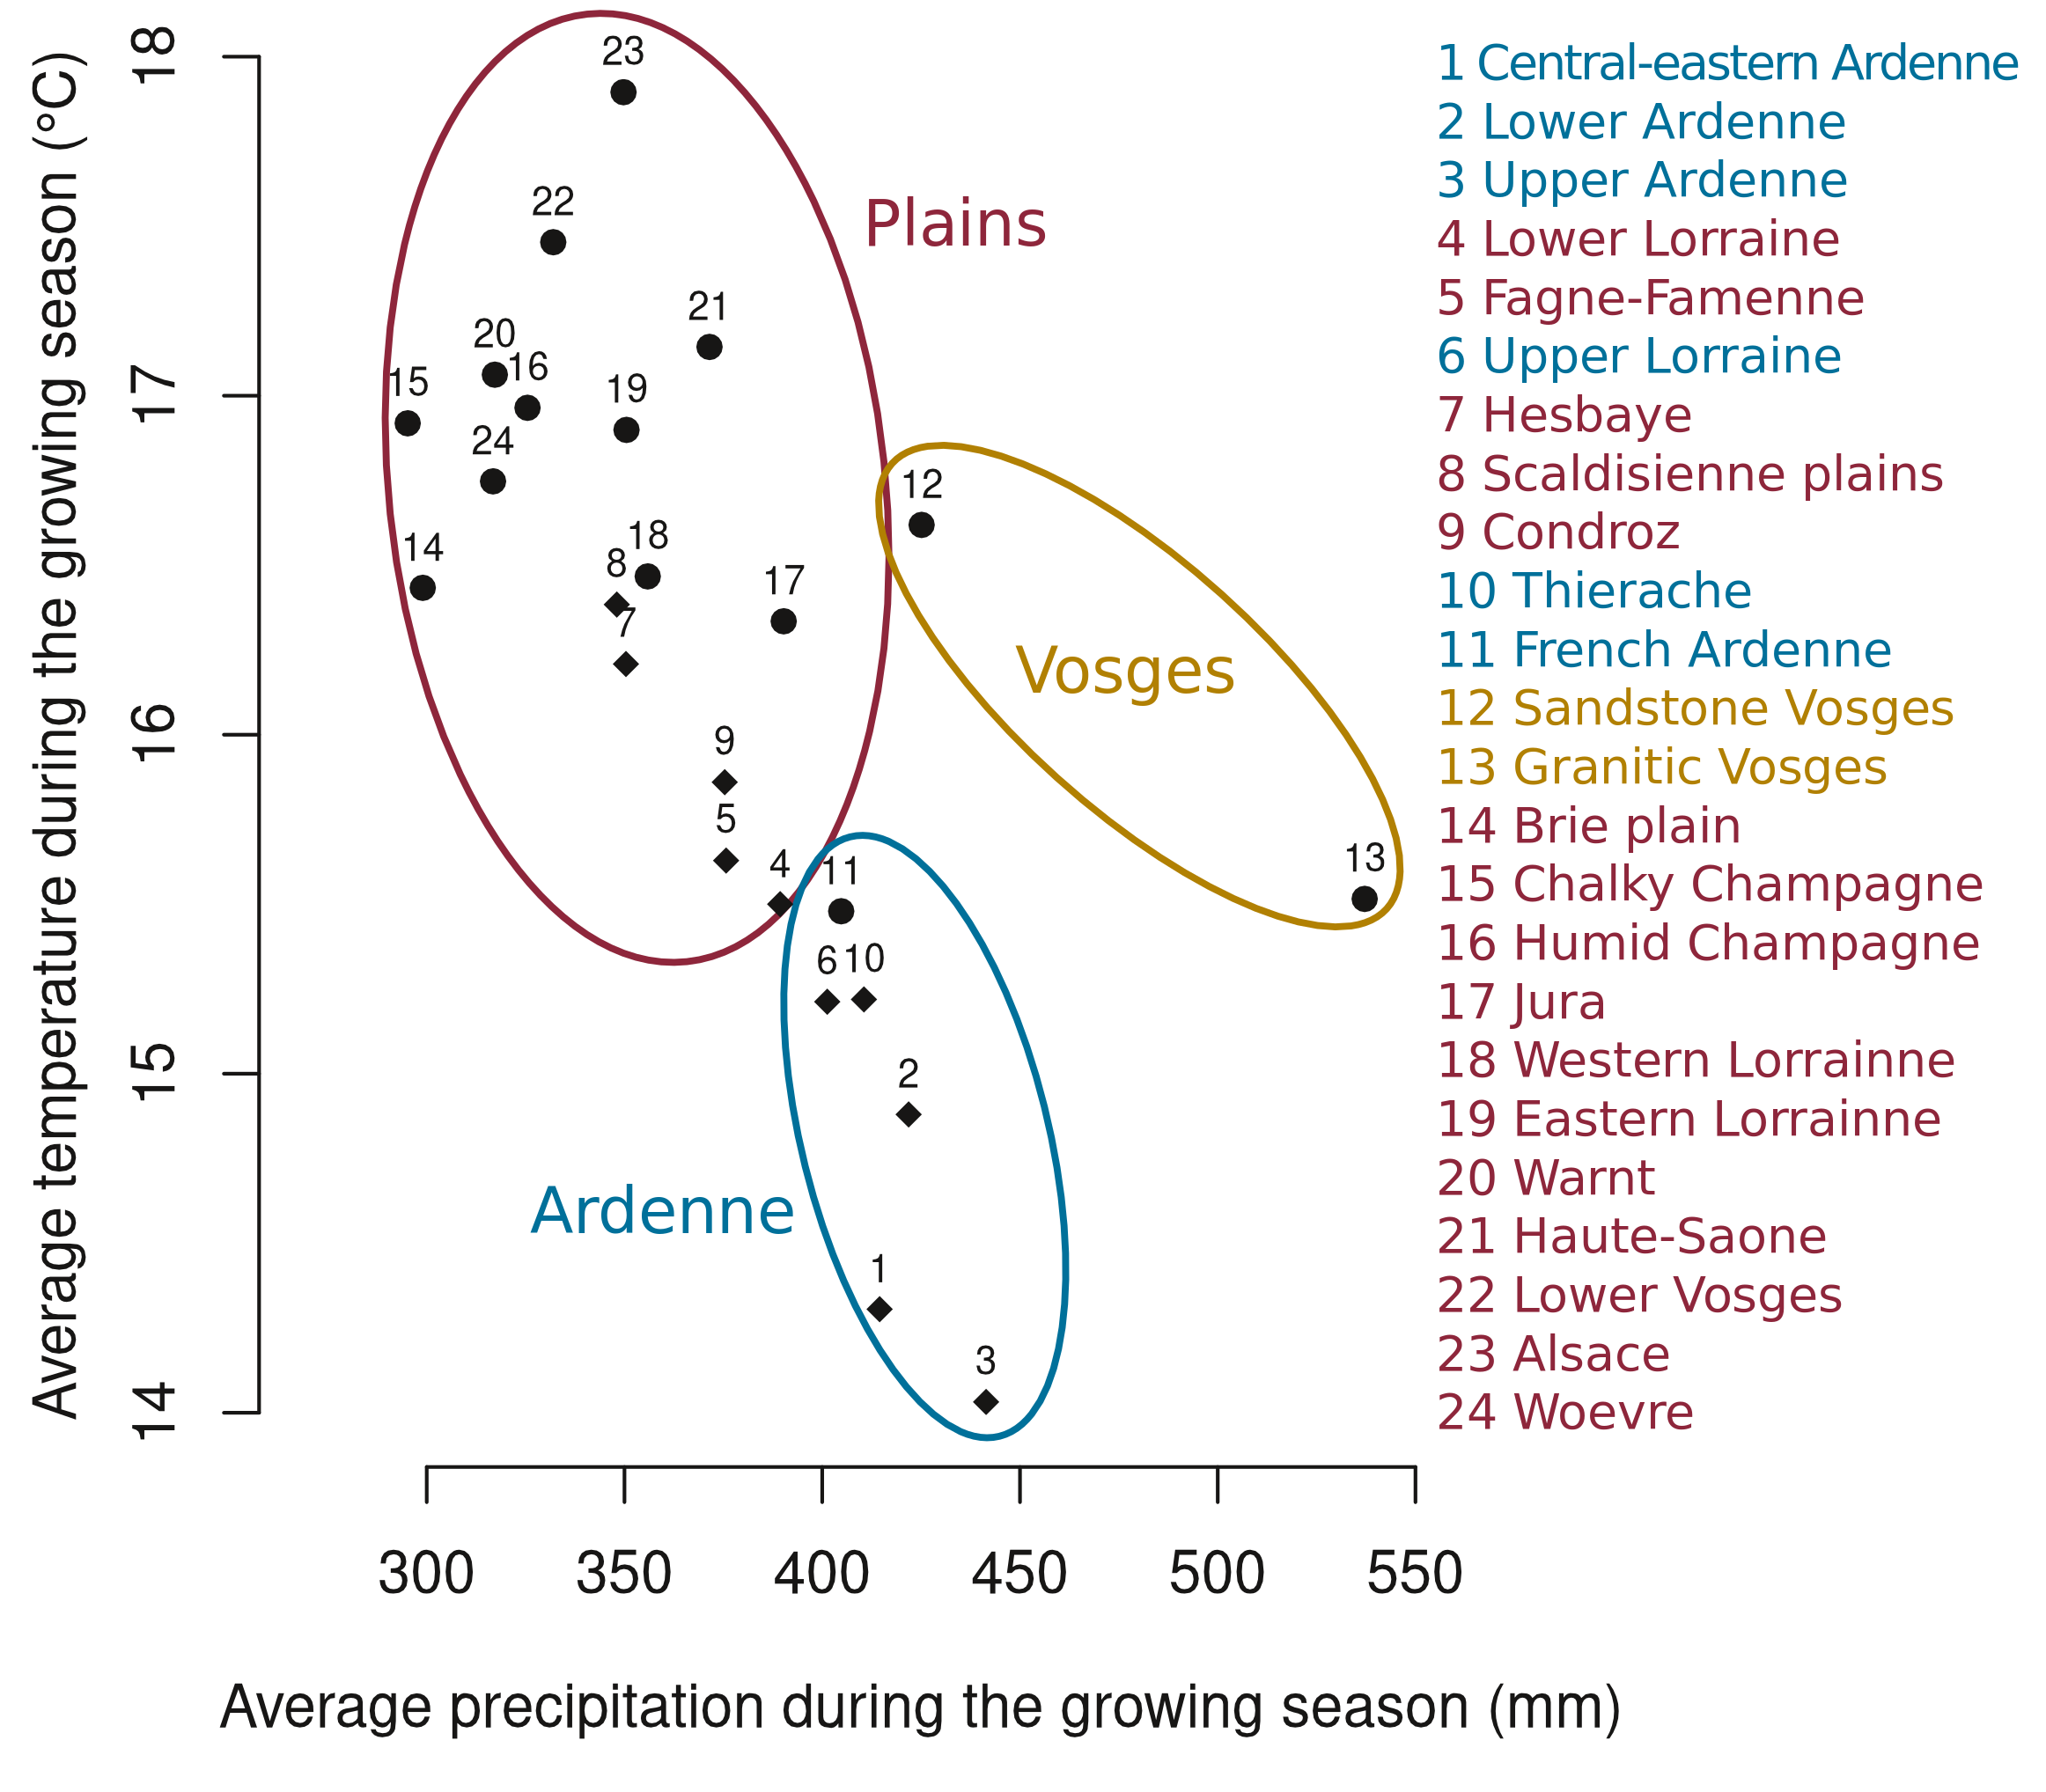
\includegraphics[width=0.8\linewidth]{climat/climat_region.png}
	\caption{Grouping of French natural regions according to the temperature and precipitation of the growing season to form three groups: Ardenne (blue), Plains (red) and Vosges (orange). Wallonia natural regions are depicted with diamond-shaped points, and Grand-Est regions are illustrated by rounded points.}
	\label{fig:clim}
\end{figure}

Forest microclimate contrast with the climate.
The micro climate is influenced including by topography \citep{de_frenne_forest_2021}.
The digital surface model data from the Copernicus Land Monitoring Service \citep{DEM_copernicus} at a resolution of 25 m have been used for altitude data's and slope calculations.
The solar orientations have been determined using the \cite{Delvaux_galoux} definition of three topographic orientations.
Plateau are neutral topographic conditions that does not create a particular micro-climate. 
North-facing orientations are slopes greater than  20\% facing north with cold and shady conditions.
South-facing orientations are slope greater than  20\% facing south with a hot micro-climate.
In this orientation the air is warmer and drier and the temperature difference between day and night is greater.
Topographic orientation maps for Wallonia and the Grand-Est have been computed with the DEM. 


\begin{figure} [htbp] 
	\centering
	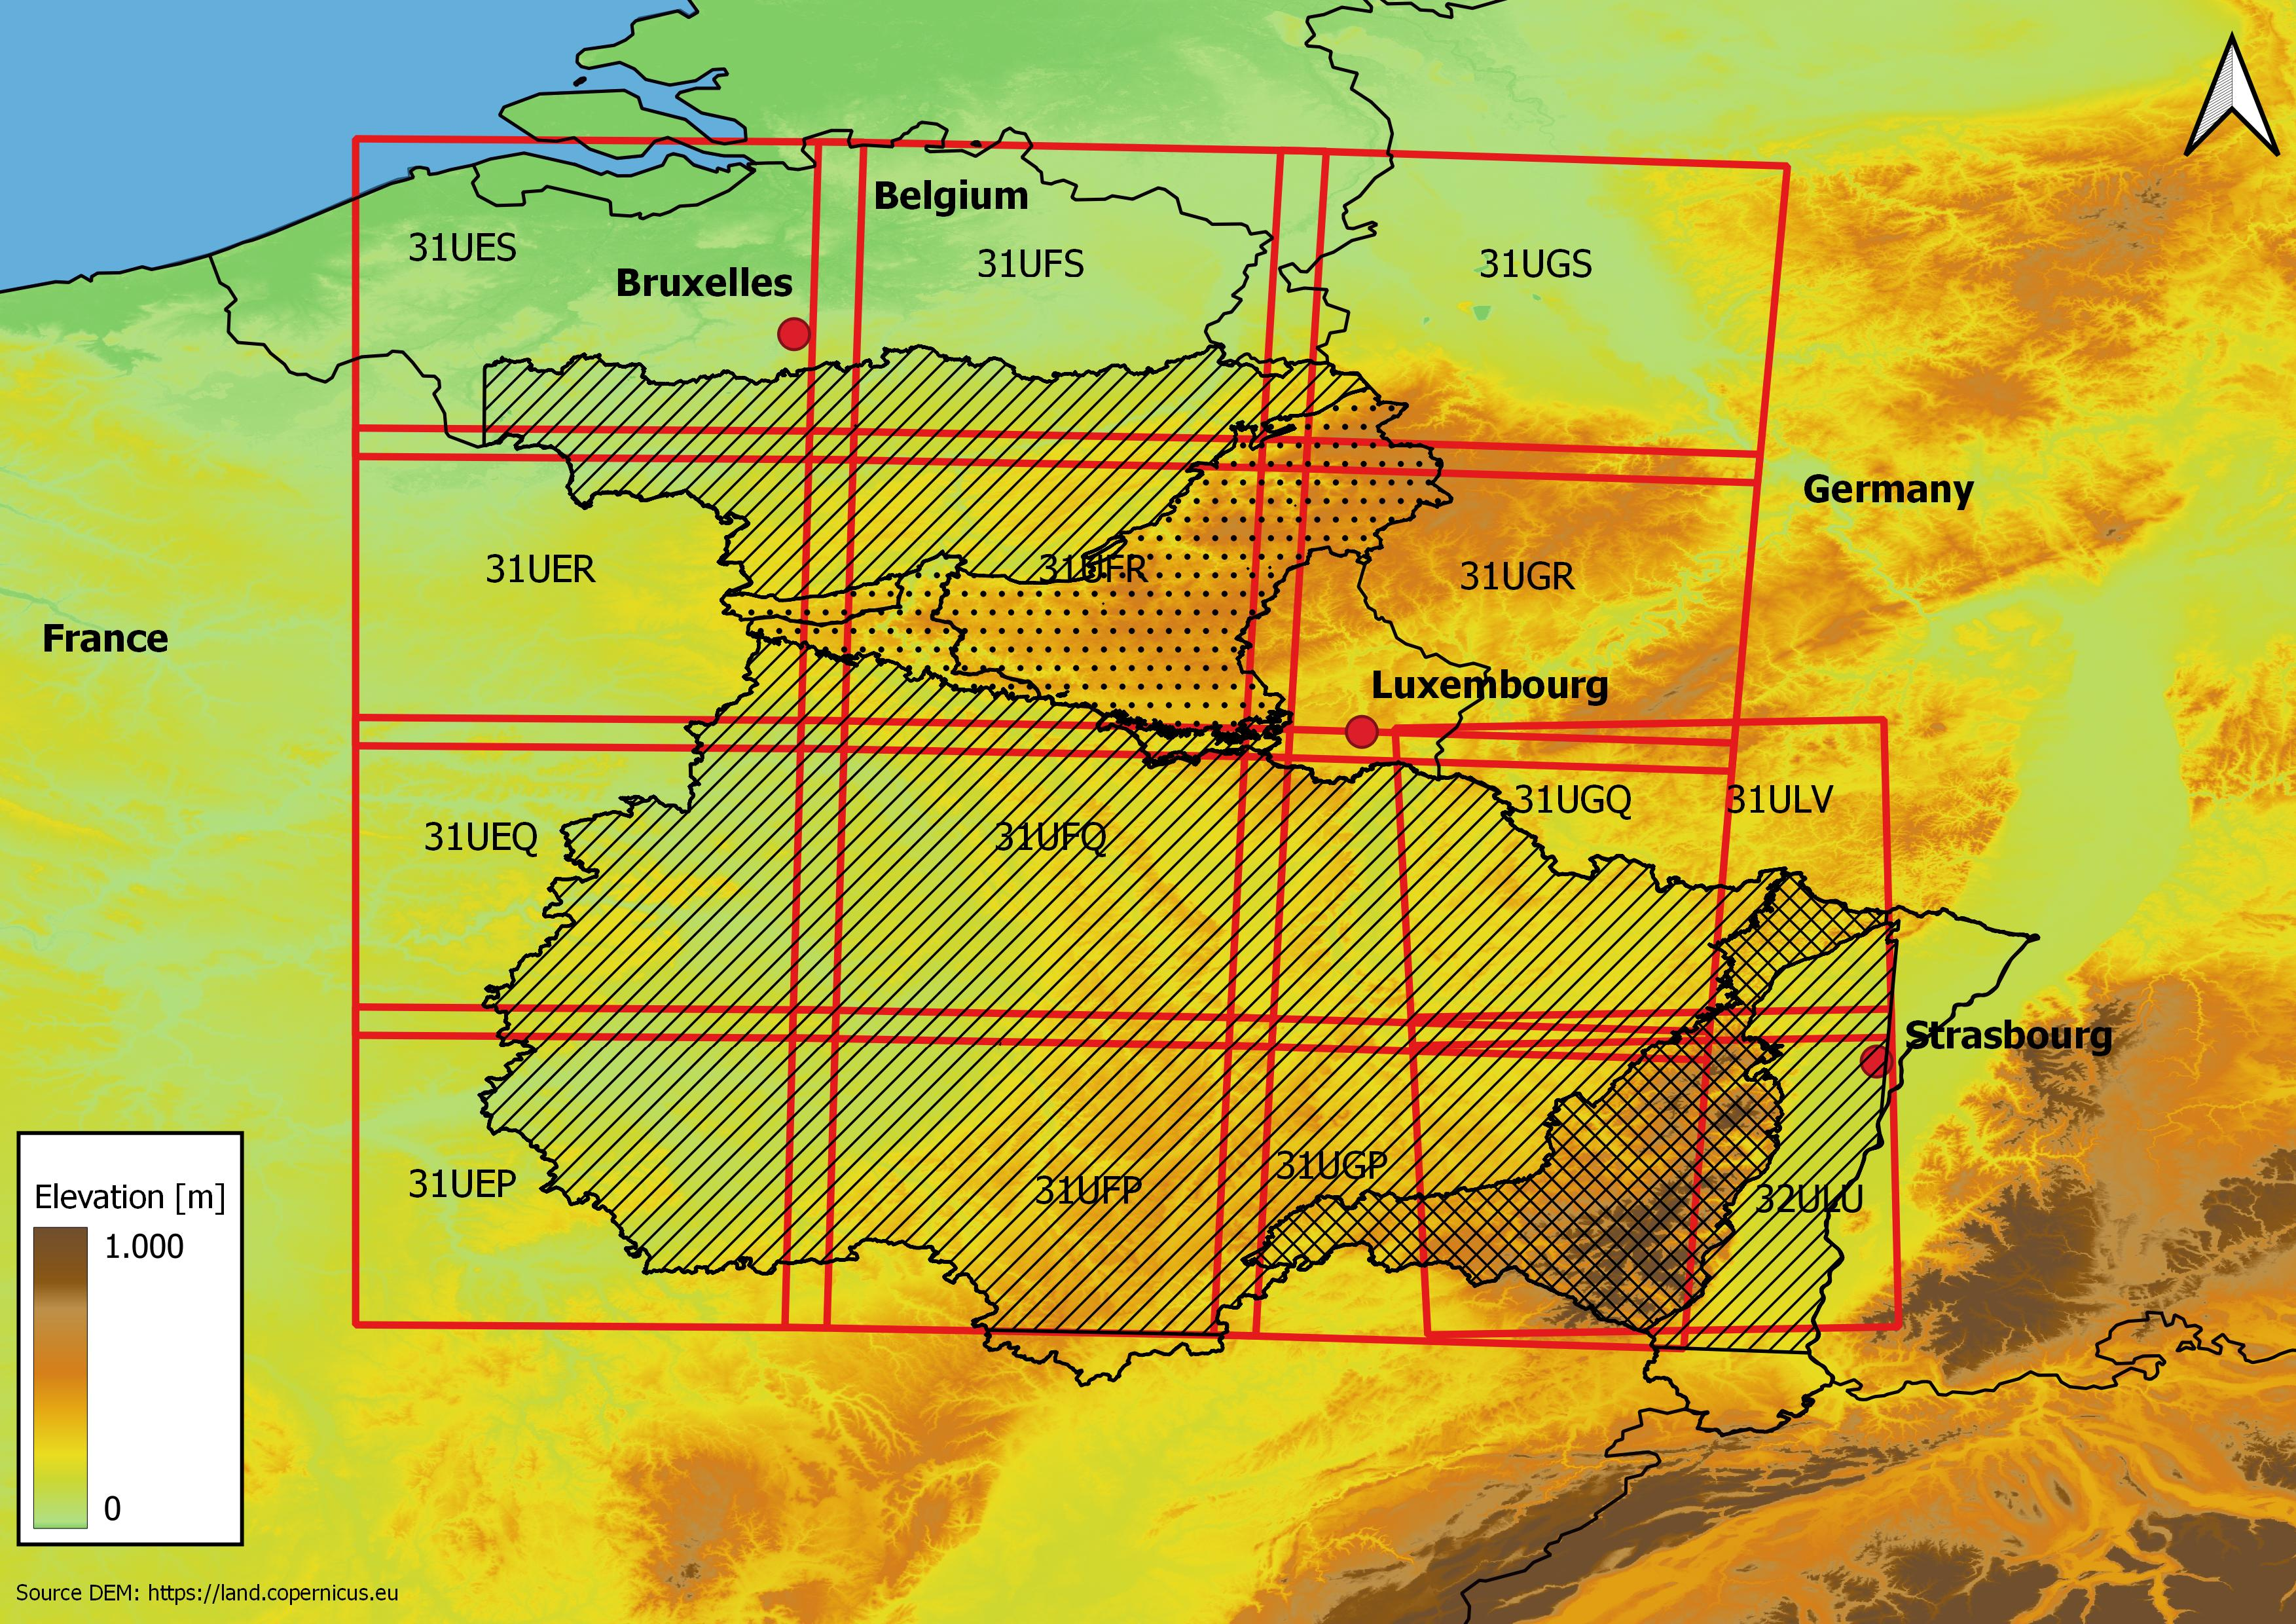
\includegraphics[width=0.8\textwidth]{gde.jpeg}
	\caption{Study area: Plains (hashed, altitude varying between 100 and 500 meters above see level), Ardenne (black dot, altitude between 100 and 700 m) and Vosges (cross, altitude ranging from 300 to 1300 m). Red squares illustrates the extend of Sentinel satellite 2 tiles which are used for the detection of bark beetle attack.}
	\label{fig:situ}
\end{figure}
%MNH

\subsection{Mapping of spruce dieback and mortality by analysis of sentinel-2 time-serie}


The detection of bark beetle infestation was realized by using dense time series of S2 imagery following the methodology developed by \cite{dutrieux_package_2021}.
Sentinel-2 (S2) satellites carry multispectral sensor with a ground resolution up to 10 m.
The three climatic areas studied are covered by 14 Sentinel-2 tiles (Figure \ref{fig:situ}).  
Vegetation changes were tracked by means of a phenology metric, the \textit{SWIR Continuum Removal} vegetation indice ($SWIR_{CR}$).
All S2 acquisitions were used in the analyses, provided that the cloud couver do not excess 35 percent. 
Bottom Of Atmosphere reflectance images (L2A product) were downloaded from the Theia data cluster \citep{theia_team} for all the 14 tiles, which size are 100km x 100km.
The $SWIR_{CR}$ is based on three spectral bands, the near-infrared, the shortwave infrared 1 band and the shortwave infrared 2, and is sensitive to the foliage water content: it is appropriated to detect spruce dieback during the green stage of bark beetle attack (Figure \ref{fig:harmo}).
Seasonal variation of $SWIR_{CR}$ for healthy stand was modelled and a bark beetle attack was detected if the observations deviates from the healthy phenology trajectory. 
Figure \ref{fig:harmo} illustrates a time-serie of $SWIR_{CR}$ observations (grey dots) for one pixel. 
In 2018, the observations went beyond the threshold represented by the purple-dashed line, which shows that the spruce stand suffer from a serious stress induced by a bark beetle attack.
A bark beetle outbreak is confirmed as soon as $SWIR_{CR}$ vegetation indice shows a stress for at least three consecutive times \cite{dutrieux_package_2021}.
In parallel to the detection of bark beetle stress, stand cutting and thinning were subject of particular attention. 
Bare soil was detected by using a combination of thresholds for red, green, blue and shortwave infrared reflectance values (Band 8A $\geq$ 12\% reflectance and Band 2 $\leq$ 6 \% reflectance and Band 3 + Band 4 $\geq$ 8 \% reflectance).
Cutting are thus taken into account and were classified either as normal harvest cutting or as sanitary thinning based on the health status prior to the cutting.
The analysis of image time-serie was thus quite straightforward and has been performed individually pixel per pixel starting from the 2016 year, which is the beginning of S2 acquisitions. 
Although \cite{dutrieux_package_2021} have published their methodology as a open-source python package, named \textit{FORDEAD}, we have adapted the pipeline in C++ in order to comply with our specific requirements (our code is online on github repository \url{https://github.com/JoLeBelge/s2-spruce-dieback/}). 
We made use of OTB toolbox \citep{grizonnet_2017_OTB} for image processing and the health status was summarized by seasonnal annual health maps (in raster format).
The annual health maps cover the vegetation period, starting from may and finishing in april of the next calendar year, because we made the assumption that Norway spruce dieback detected in april are related to bark beetle attack from the previous calendar year \citep{muller_features_2022}.
For every years between 2018 and 2021, the heath state of every single pixel located in a spruce stand is summarized in one of the four following classes ; healthy, bark beetle attacked, cutted or sanitary thinning.
The dense time-serie covers the 2016-2021 period and count a minimum of 180 acquisition dates. 


\begin{figure}[htbp] 
	\centering
	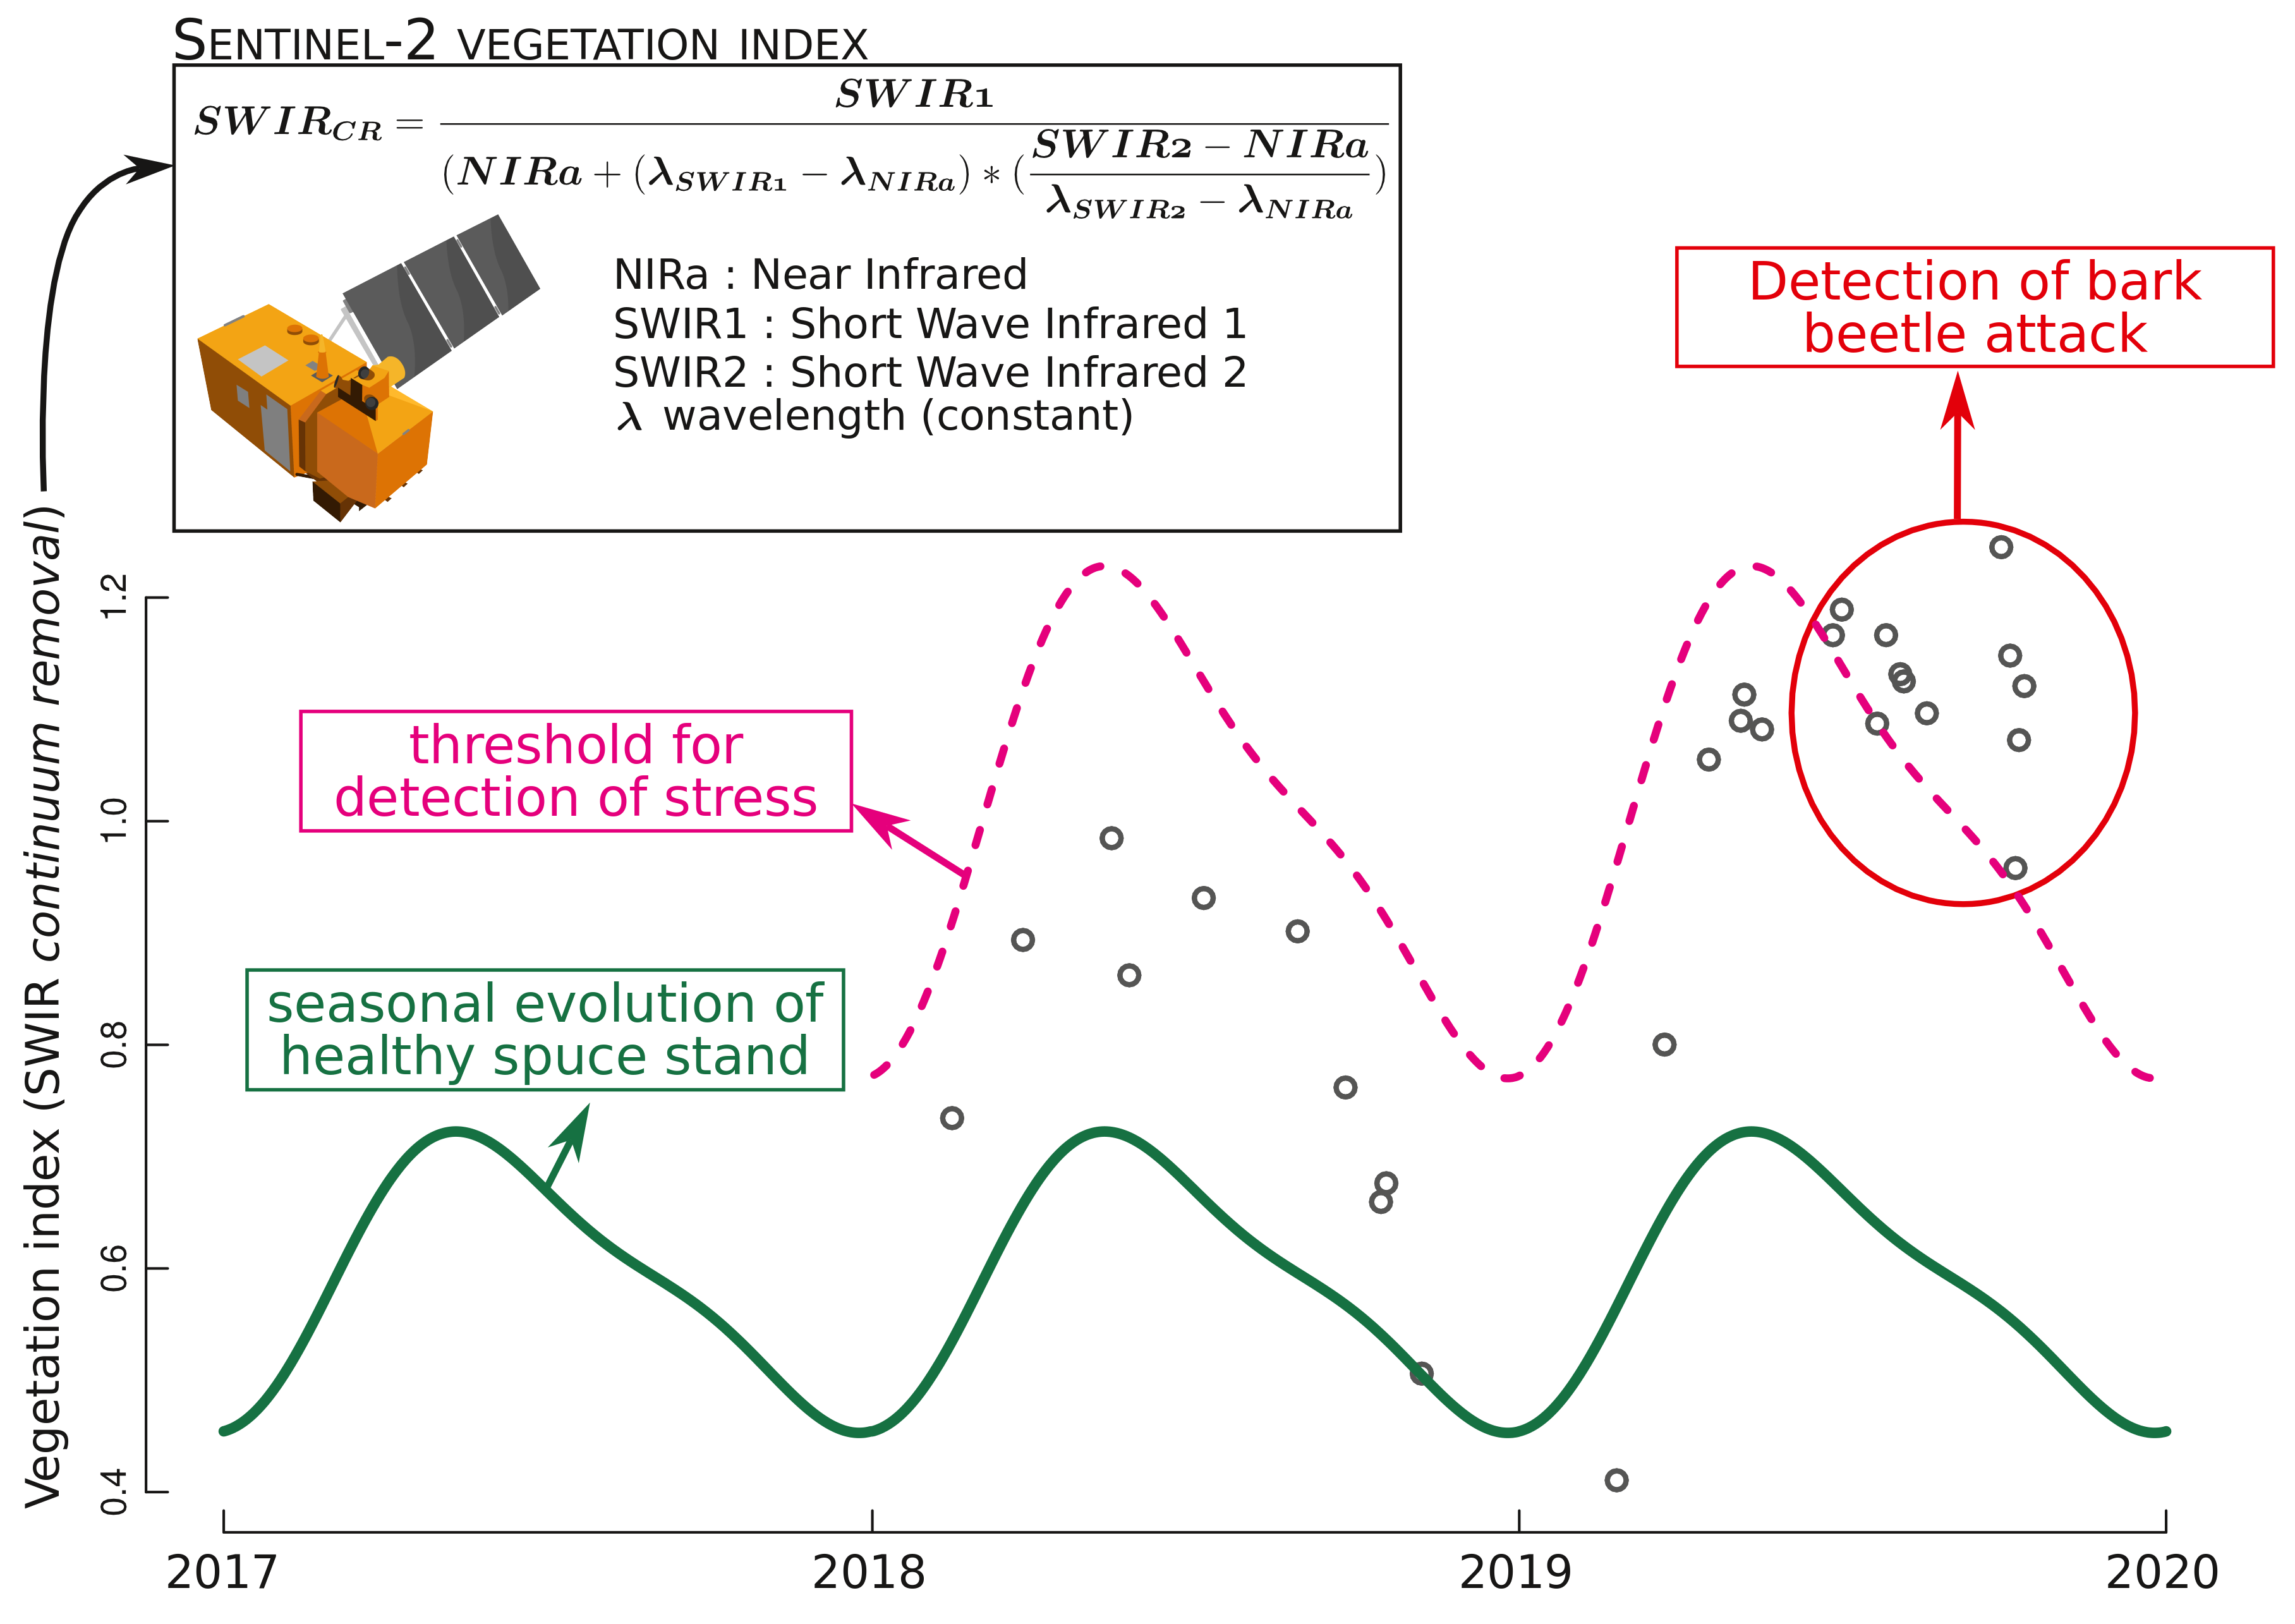
\includegraphics[width=0.8\textwidth]{fctHarmo.png}
	\caption{Bark beetle infestation map are computed by detecting change in the $SWIR_{CR}$ phenology metric. The \textit{SWIR Continuum Removal} is computed using three bands from Sentinel-2 imagery for every single acquisition date and his value is compared to a threshold (purple dashed line) in order to detect vegetation stress. If a stress is detected three consecutive times, we assume that a bark beetle infection occured.}
	\label{fig:harmo}
\end{figure}

Our approach of dieback detection is only suitable for Norway spruce, as it is closely related to the phenological course of healthy spruce forest.
An essential prerequisite was thus to have a proper mapping of spruce stands.
For the south of Belgium, we used existing reliable composition maps from \cite{bolyn_mapping_2022}, computed from remote sensing data, in order to restrict our analysis to Norway spruces.
In the Grand-Est, the composition map came from the French mapping agency \citep{IGN_bd_2018}. 
Composition of forest stand was determined by photointerpretation and forest stands identifyed as "spruce or fir" served as starting point to restrict the dieback analysis.
Time series are a convenient means to track phenology changes. 
More broadly than the dectection of bark beetle infestion, phenology courses are highly suitable for forest tree species discrimination \citep{lisein_discrimination_2015,grabska_forest_2019,ma_tree_2021}.
We have used S2 spectral bands courses along the vegetation season to refine the determination of species present in the area interpreted as "spruce or fir" in Vosges.
The objective was to identify and remove every area that did not correspond to spruce stand, as pixels located on others species than spruce were likely to be wrongly detected as a bark beetle attack.
All S2 spectral bands were first summarized for each of the four trimesters of the year, by simply averaging all observations occuring during the trimester.
Then, a Random Forest algorithm was trained on these synthetic intra-annual time serie to discriminate spruce from non-spruce pixels, based on a training set of observation from Belgium \citep{bolyn_forest_2018}.
Eventually, this Random Forest classifier was applied on "spruce and fir" area of Vosges and bark beetle detection was carried on only for pixels detected as spruce. 

The maps were validated by two different methods on the Wallonia.
The first method is global validation with annual orthophotoplan on random spruce stand on the 2018-2021 period. 
For the second method, a stratified random sampling base on  the siz of the spruce stand was used for 2018. 
The selected stands were photo-interpreted with the annual orthophotoplan of the Wallonia.



\subsection{Relation between bark beetle attack and environmental condition}



%To select important variables that influence the Norway spruce dieback, we use the the random forest algorithm \citep{genuer_vsurf_2015} in Wallonia.
%We apply the random forest only in Wallonia.
%Individual classification trees are trained on a 500 samples of dead spruce stand of 0,25 Ha and 500 samples of healthy stand by randomly selecting a subset of explanatory variables (topographic and  climate variable).

The forest practitioners of the two countries drew our attention to the variables that seemed to influence spruce dieback.
According to them, the south-facing slope and altitude influence the dieback.
In Western Europe, altitude reflects the climate. Precipitation increase with altitude and and conversely, temperatures decrease the higher the altitude.
The Norway spruce spruce need amount precipitation to grow correctly.
The south- facing slope are warmer than other topographic orientations, the bark beetle 
population develop favorably with heat \citep{annila_influence_1969, baier_phenipscomprehensive_2007, jonsson_2009, marini_climate_2012} and increase the susceptibility of Norway spruce to the attack of bark beetle \citep{wermelinger_ecology_2004, netherer_waterlimiting_2015}.
If we follow this theory, there should be more dead Norway spruce in low altitude and in south-facing slope in the three climatic areas.  
Sanitary map have been used to study the relation between the dieback and this two topographic variables.
%climat proxi altitude 
%altitude facile à avoir sur deux pays à haute resolution
%Microclimat ss 
% basse altitude % Sous secteur chaud  + plus chaud - de pluies don cfavorable aux scolyte et defavorable àl'épicéa
% Sous secteur chaud 
The altitude has been broke down  by 100 m classes and kept the three topographic orientation classes.
Then, in order to determine the classes of these factors most impacted by the bark beetle, we estimated the bark beetle areas for each class of each factor based on the health status maps for each year of the period 2017-2021.
The dieback ratio is  the dieback area of a class during one year divide by the total area of Norway spruce of this class at the beginning of the same year. 
Dieback area is the surface of Norway spruce attacked by bark beetle and the area of sanitary cutting during the year. 
The total area of spruce at the beginning of the years is composed of the area of healthy spruce area at the beginning of the year. 


%mettre equation 
%\[
%\frac{\sum dead\, spruce\, area\, of\, the\, year }{\sum spruce\, area\, at\, the\, beginning\, of\, the\, year\,}\]

The spruce area studied is 120,365 ha in Ardenne, 24,462 ha in the Vosges and 75.067 ha in the Plains in the Grand-Est region.

  
			
% Classe d'latitude
%calcul prob prese
%Comparaison entre le différents pays
%Depuis 2018, des attaques massives de scolytes tuant les épicéas frappent la Wallonie. Suite à ces évenements,les forestiers se sont interrogés sur cerains facteurs topographiques semblant avoir fortement influencé les attaques de scolytes.
%Les pessières situées en basse altitude semblent avoir été plus touché ainsi que les peuplement situé sur des versants sud.

%Pour caracteriser les attaques de scolytes, nous avons appliquer la méthode des random forest afin de selectionner les 2 facteurs topographiques influençant le plus les attaques de scolytes. CEs deux facteur sont l'altitude et les sous-radiatif. Nous avons ventilé l'altitude par classe de 100m et conservé les trois classes de sous secteurs définis par delvaux et galoux.

%Ensuite, afin de determiner les classes de ces facteurs les plus impactés par le scolyte, nous avons estimé les surfaces scolytés pour chacune des classes de chaque facteurs sur base des cartes d'état sanitaire pour chaque année de la période 2016-2021.

%La carte d'etat sanitaire de la pessière a été subdivisée en tuile de 50*50m (25 pixel de 10X10m) comprenant au minimum 17 pixel de 10mX10m d'épicéas. Une tuile est considérée comme %scolytée quand minimum 3 pixels sur 25 sont scolytés.

%Pour chaque tuile, la classe d'altitude et le sous-secteur ont été extraits.

%Nous avons calculé le ratio du nombre tuiles scolyté d'une classe divisé par le nombre total de tuiles de la classe (probabilité de présence) pour chacune des classes d'altitude et de sous-secteurs.


%\begin{align*}

%$presence\,of\,probability = \frac{tiles\, affected\, by\, the\, bark\, beetle\, of\, a\, class}{total\, number\, of\, tiles\, in\, the\, class}$

%\end{align*}



%However, other factors such as degres day data could influence bark beetle attacks 
%We made a selection of factors influencing bark beetles favourably and norway spruce unfavourably using the random forest method. The factors emerging from this analysis show that altitude and radiative topography orientation are the most important factors 






\section{Results}

%\subsection{Choice of environmental variable}
%The altitude and the topographic orientation were selected as explanatory variable by the random forest algorithm.
%We study the dieback of the Norway spruce in function of this two variables.



\subsection{Evolution of the dieback }

The drought touched the western Europe since 2018.
However, the outbreaks did not occur at the same time in the different region (Figure \ref{evol_gen}).
The first major dieback took place in the Ardenne in 2018 but the peak is directly reached and a decrease of dieback ratio is observed in 2019. 
A slight recovery in dieback occurs in 2020.
%add reference crise 5 ans
The area of Norway spruce killed in Ardenne during the five years of the study is 22.520 ha.
The maximum of the ratio of area touched by bark beetles during crisis peak in 2018 is 8,4\%. 
The climatic area of the Ardenne have lost 18,7 \% of his Norway spruce area.
In the Vosges, there is 4.248 ha killed by bark beetle.
However, the maximum ratio of area affected by this insect is 2,8 \% in 2020.
The Norway spruce stand of the Vosges climatic has been reduced of 5,6 \% of his area. 
At the peak of the crisis the Vosges are proportionally less affected than the Ardenne.
The important damage of the Plains spruce stand have begun in 2018.  
The Plains climatic area is  with the most area and proportion of area affected.
This regions have three times more area touched by bark beetle than the Vosges.
The Plains region reached the maximum of area affected by bark beetles in 2020. 
The peak of proportion of area impacted is reached at 22 \%.
In total, more than half of the spruce stands were affected by bark beetles in this area.
The area killed by this resinous pest is detailed in table \ref{tab_recap}.
% add syrface


\begin{table}[htbp]
 \caption{Summary table of the crisis }
 \label{tab_recap}
\begin{tabular}{|l|l|l|}
\hline
Region   & \begin{tabular}[c]{@{}l@{}}Total Norway spruce \\ area killed (2017-2021)\end{tabular} & \begin{tabular}[c]{@{}l@{}}Total Norway spruce \\ area before crisis\end{tabular} \\ \hline
Plains  & 12.723 ha                                                                                              & 24.462 ha                                                                         \\ \hline
Ardenne & 22.520 ha                                                                                              & 120.365 ha                                                                        \\ \hline
Vosges   & 4.248 ha                                                                                               & 75.067 ha                                                                        \\ \hline
\end{tabular}
\end{table}




%The evolution of the crisis differs between these two neighbouring regions.

%In Wallonia, during the year 2017 and 2018, there are already norway spruce affected by bark beetle in low elevation but the probability of presence is under 10\%. 
%In 2019, the peak is reached in all of classe of elevation. During this year, the percentage of area of the Wallon norway spruce stand affected by bark beetle is 2.8\%.
%In 2020, there a  little diminution of attack. 
%During 2021, there are important diminution of area impacted by bark beetle. The probability of bark beetle presence returns to the same level as begin the crisis.

%In Grand-Est, during 2017, the attack of bark beetle are weak. 
%In 2018, there are first attack at low elevation but always below 5\%.
%In 2019, the increasing of attack at low altitude continues.
%In 2020, in all altitude classes are impacted by bark beetle. 
%Between 100m an 400m of altitude there are a important augmentation of the probability of presence. 
%The maximum of area affected is reached. % indiqué pourcentage max atteint
%During 2020, there is 4\% of the total area of spruce stand of Grand-Est that area affected by bark beetle during 2020.
\begin{figure}[htbp] 
   \centering
   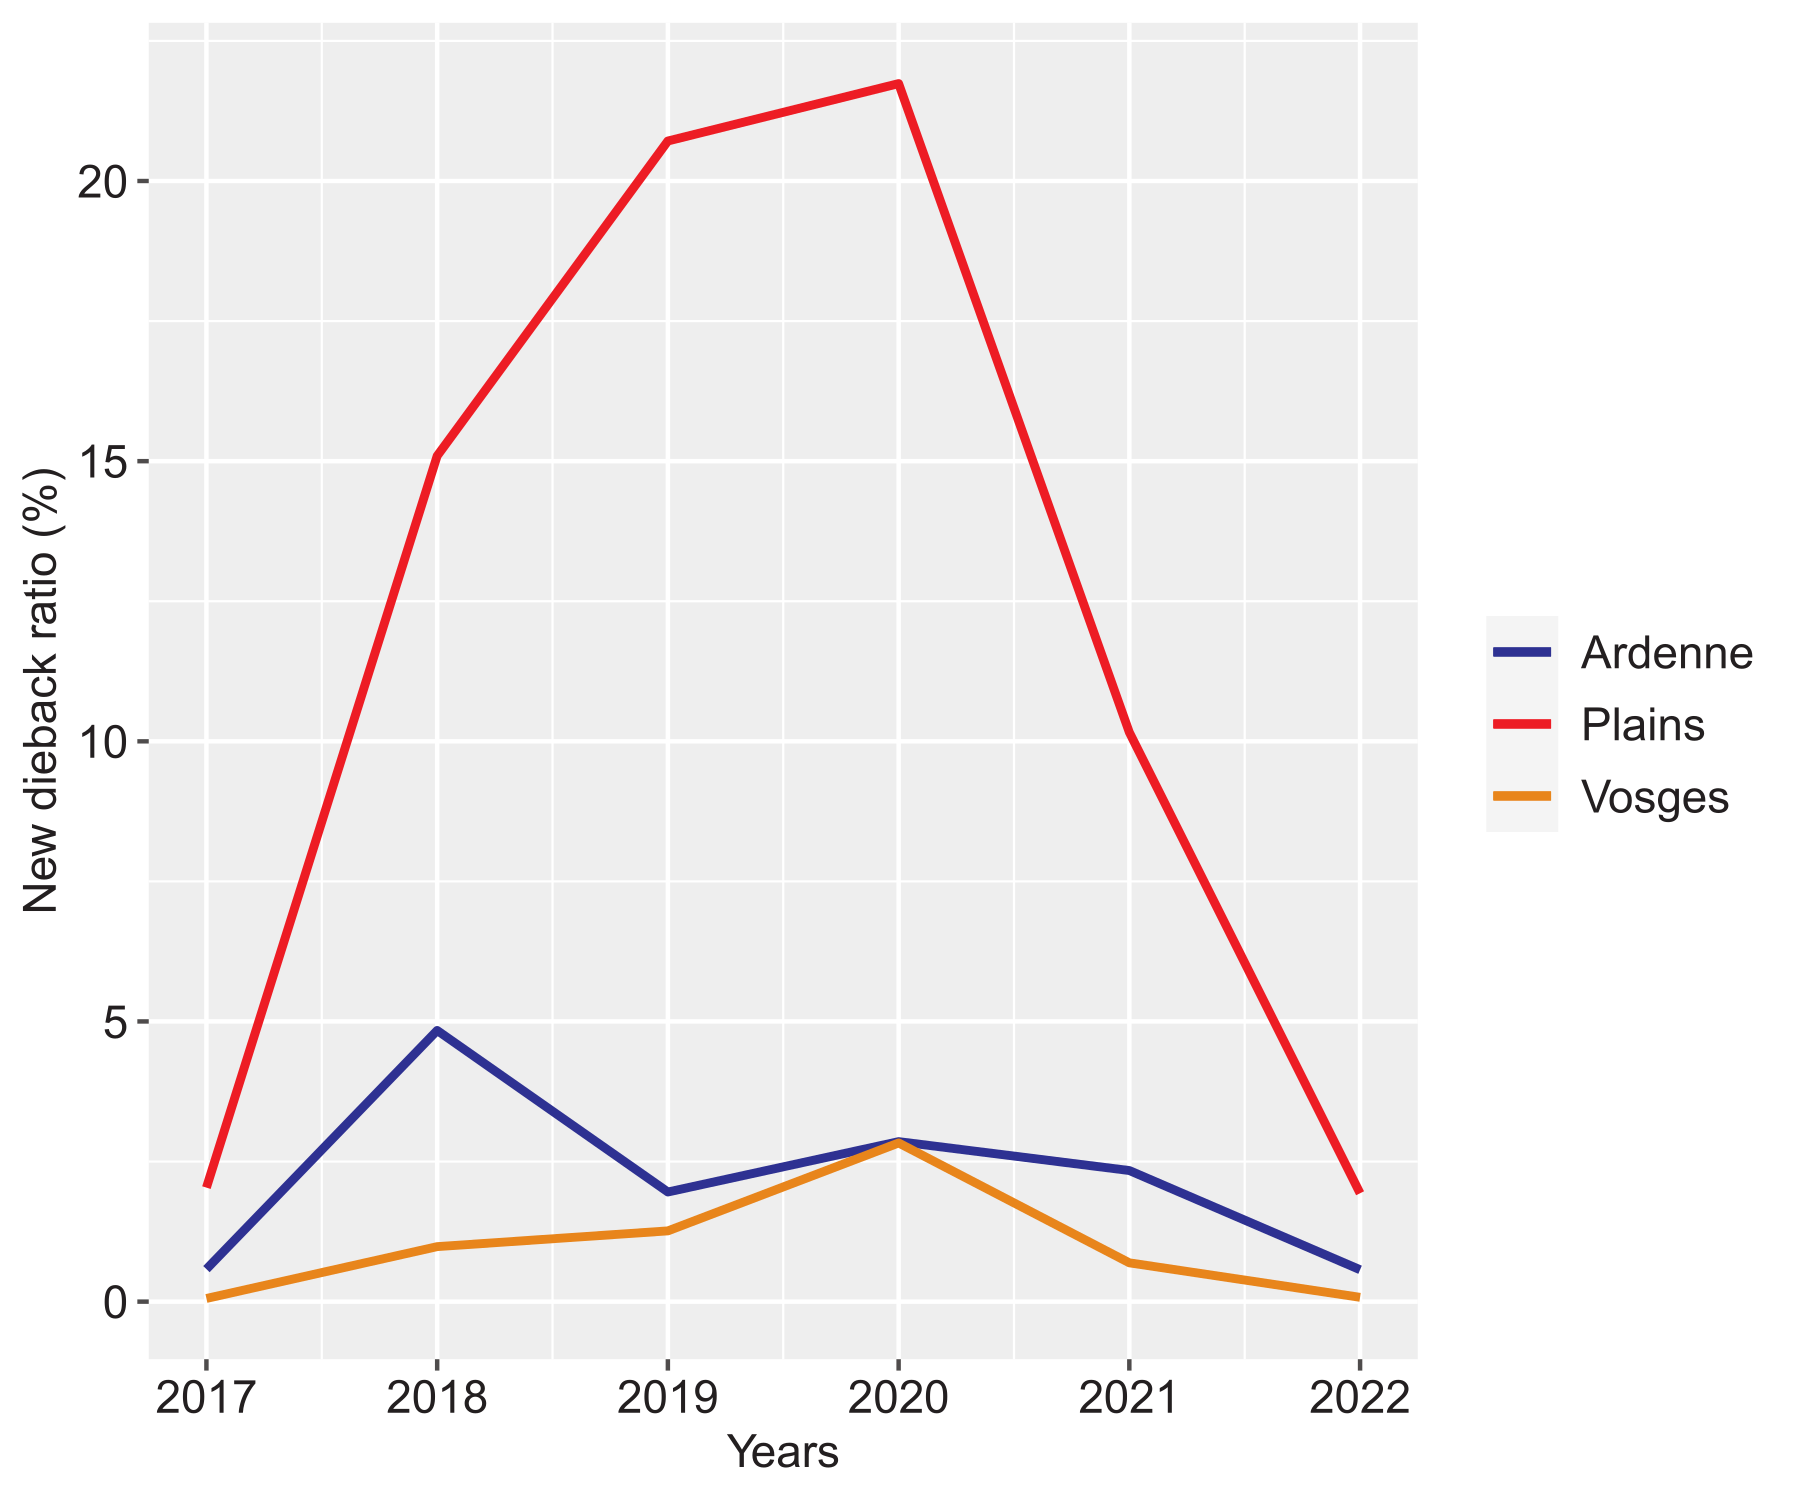
\includegraphics[width=0.6 \textwidth]{Annual_evol_Ardennes_vosges_plaines.png}
    \caption{Proportion of Norway spruce area affected by bark beetle. Plains region in red, Ardenne in blue and Vosges in }
    \label{evol_gen}
\end{figure}

    


\subsection{ Influence of altitude on the Norway spruce dieback}
The altitude is easily usable for the forest manager.
The precipitation in western Europe depend of altitude. 
The majority of spruce in the Plains is located in low altitude under 400m of altitude in contrast with the Ardenne and the Vosges where the majority of Norway spruce stand grow above 400 m. 
The variation of the dieback ratio in the three climatic areas for the period 2017-2021 is described in the Figure \ref{alti_sco}.
%The altitude has been subdivided into the same 12 elevation classes for both regions. 
%The graphs corresponding to the variation of the probability of presence in Wallonia are in the upper part of the figure and those for the Grand-Est in the lower part.

\begin{figure}[htbp] 
\centering
	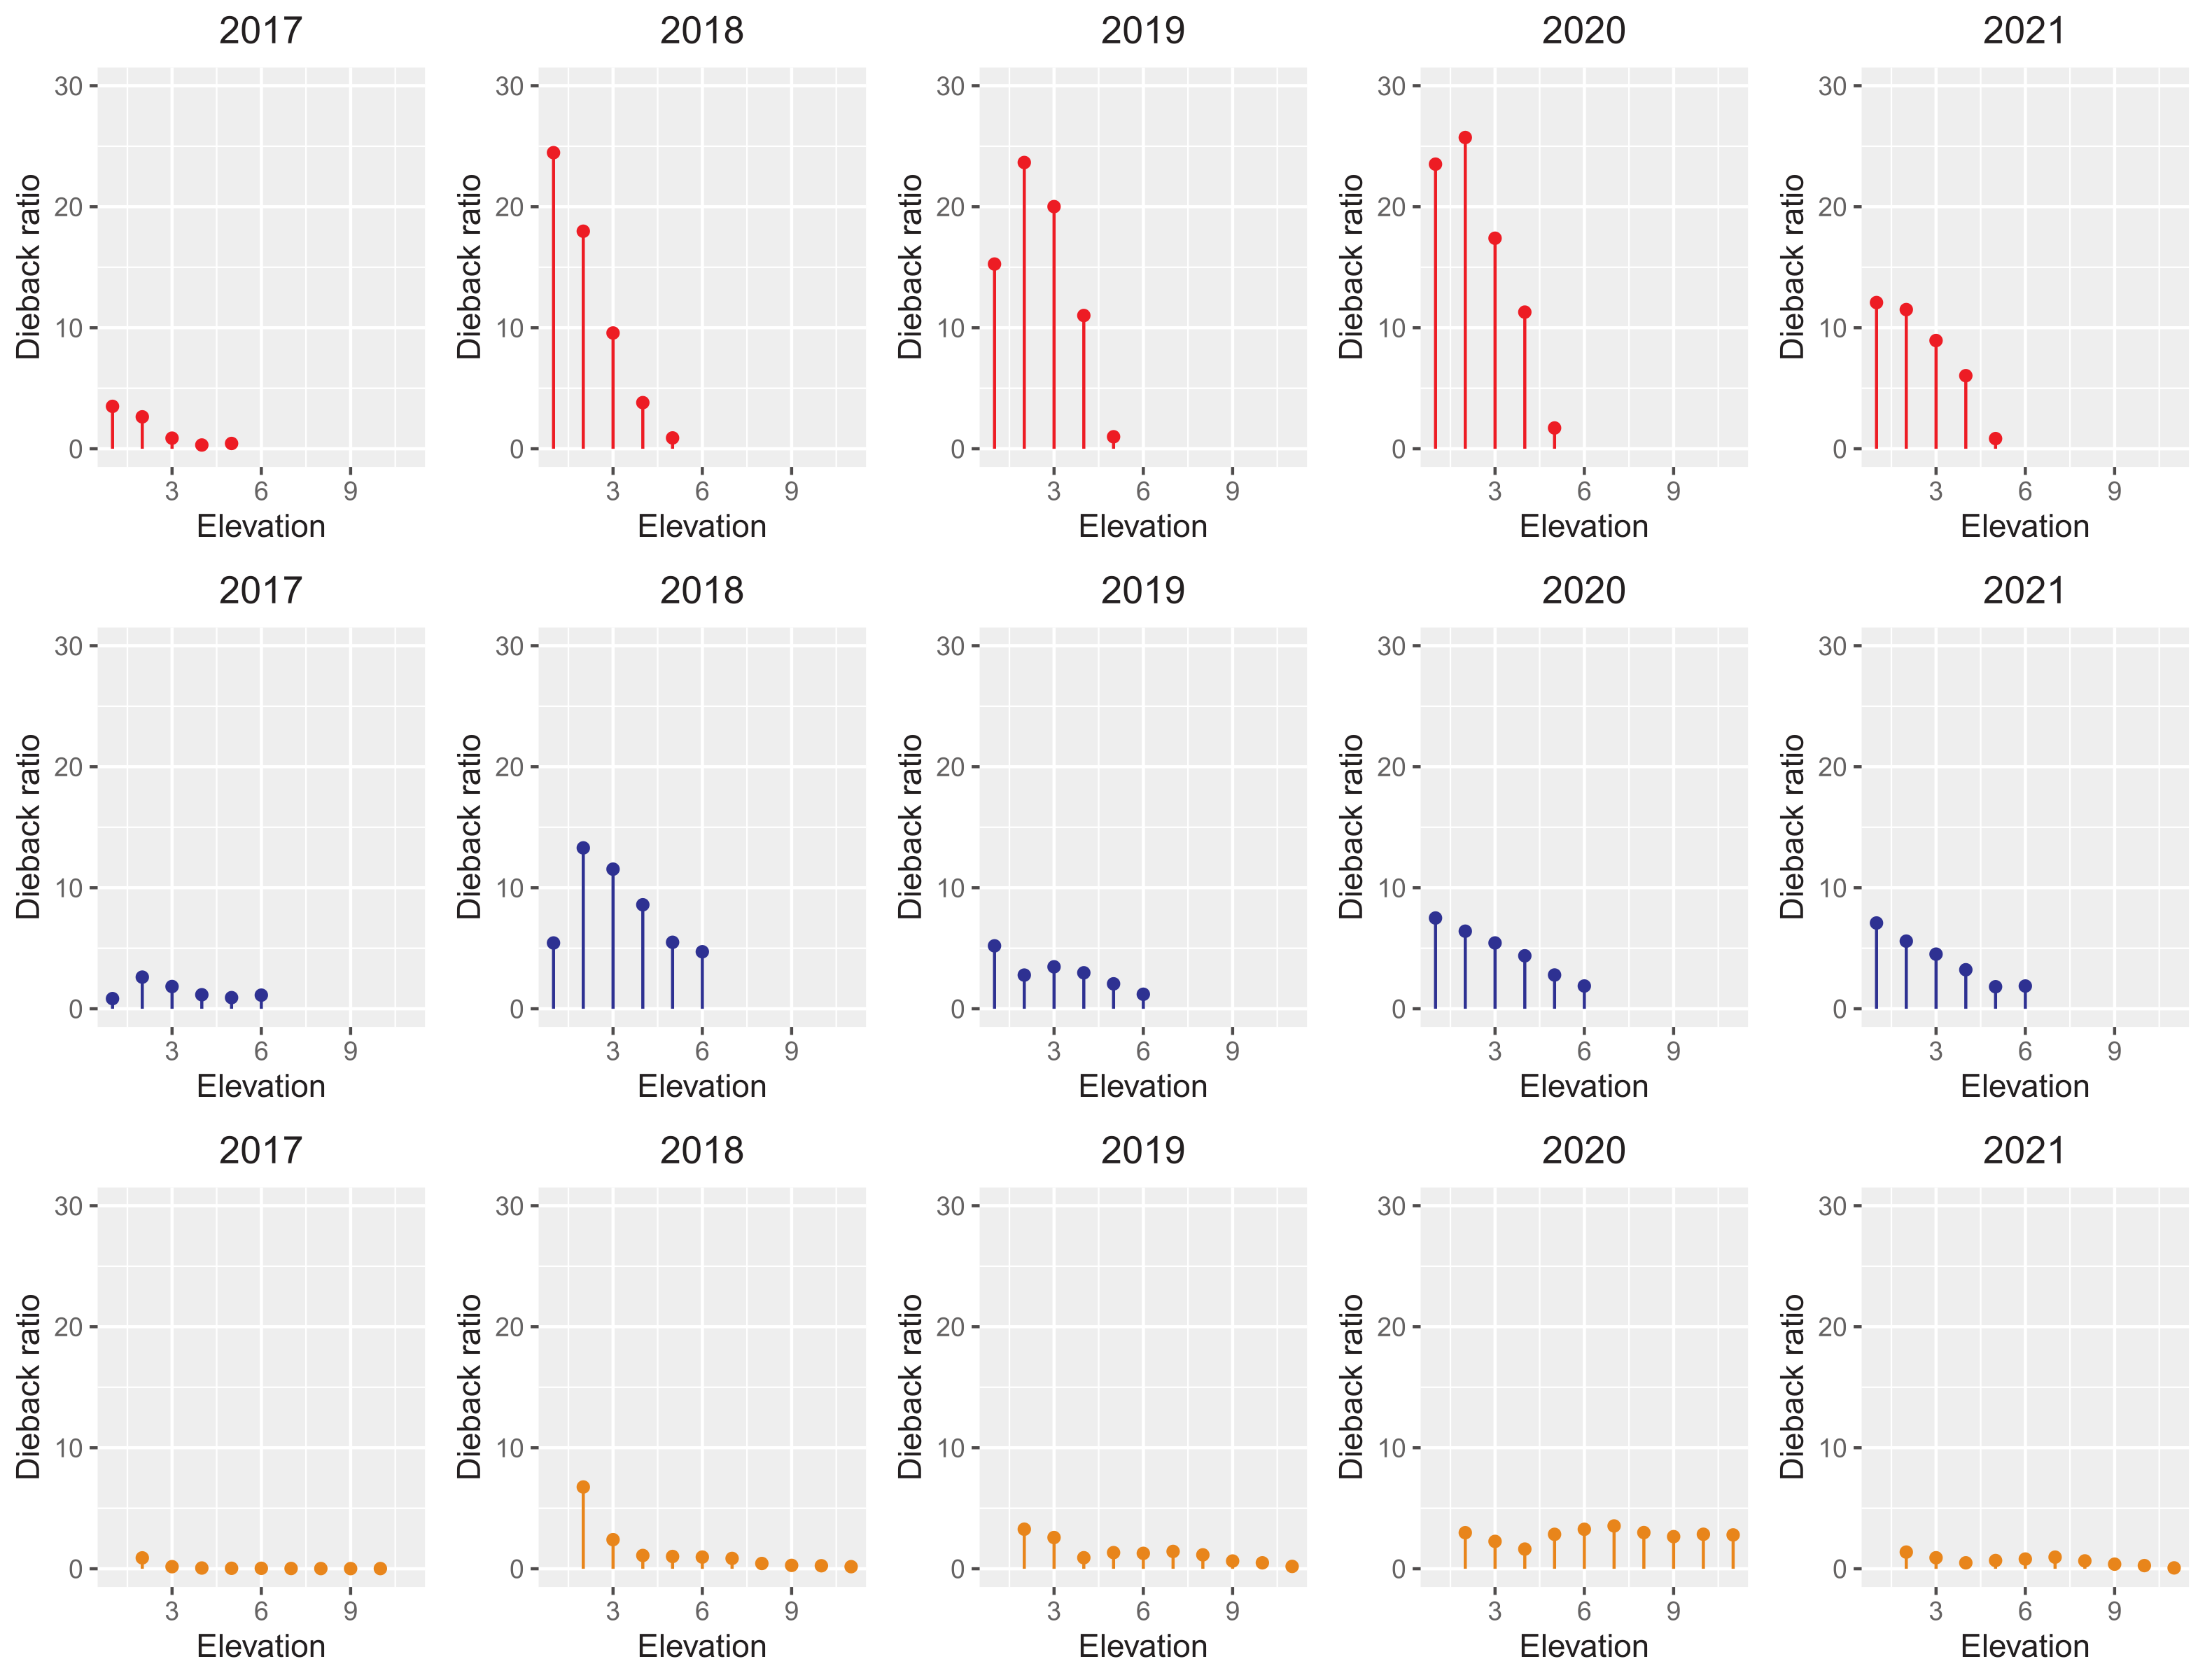
\includegraphics[width=\textwidth]{synthese_color_11_2022.png}
     \caption{The altitude has been subdivided into the same 12 altitude classes for the three regions. 
The graphs corresponding to the variation of the dieback in Ardenne (blue) are in the upper part of the Figure,the Vosges (Orange) in middle part and for the Plains (red) in the lower part.
}
	\label{alti_sco}
\end{figure}

In Ardenne group, in the begin of the crisis, the low altitude classes are more affect than hight altitude classes.
The dieback of Norway spruce occur along a altitudinal  gradient.
This gradient is confirmed over the 5 years of the study.
Indeed, during 2018, there is a strong increase of the dieback ratio in the 100-200m and 200-300m altitude classes is observed. 
These two altitude classes are more affected during the crisis.
The stand located above 400m are weakly attacked with maximum 8,6\% in 2018.
In Vosges group, all of the altitude classes are affected by dieback in a similar way.
No trend seems to emerge.
The low altitude are poorly represented. 
There are no impact of altitude on the presence of bark beetle. 
The dieback ratio is inferior of 5 \% during the study period.
The Plains group are affected mainly in low altitude with a hight dieback ratio. 
During the crisis the class of altitude 100 m-200 m et 200 m-300 m are strongly affected with a probability of presence exceeding 20\%.
There is also like in the Ardenne group, a diminution the dieback along a altitudinal gradient.
The low altitude stand are the more affected stand and are disappearing.
During the five crisis year, the trend are similar for the two climatic areas that have the maximum elevation under 700 m, there dieback ratio the ratio is higher at lower altitudes. 
The dieback of Norway spruce in the Vosges climatic area is not influenced by the variation of altitude.


%The decrease the probabilty of bark beetle presence follow an altitudinal gradient.
%The higher the norway spruce stand grows at an altitude, the lower the probabilty of bark beetle presence. 
%For the Grand-Est region, there is an increase in the probability of bark beetle presence between 2019 and 2021. 

%In the Grand-Est stand, the situation differs than is neighbour region. In 2017, there is low presence of bark beetle  at all altitude.
%The crisis begin weakly in 2018 with attack at low altitude.
%However the probability of presence of bark beetle increase until 2020 to reach more than 20\% of norway spruce killed at altitude below 300m.
%Above 400m, the decreasing didn't follow a altitudinal gradient.
%The probability of presence of bark beetle is relatively constant with a little increase between 700-800m.
%Above 400m, the altitude didn't protect spruce against bark beetle attack in the Grand-Est.

%Unlike the Walloon spruce forest, there is no clear altitudinal gradient in the Vosges. 
%As in Wallonia, the 200-300m altitude class is strongly affected by the bark beetle. The probability of presence decreases along an altitudinal gradient between the altitude classes 200-300 and 400-500m. However, above 500m the probability of bark beetle increases up to the altitude class 700-800m.
%_Description figure \ref{fig:sco_alti} 
% augmentation de la probabilité de présence jusqu'en 2020 et diminution en 2021
% Wallonie: Diminution de la probabilité de présence de scolyte avec l'augmentation de l'altitude 
% Vosges pas de relation clair avec l'altitude. Cependant, les classes d'altitude 2, 11 et 12 semblent + touchées que les autres classes d'altitude
% et ne pas oubnlier de citer untel et machin
	
% Wallonie + Vosges: Augmentation de la probabilité de présence de scolyte avec le temps quelque soit la classe d'altitude.


\subsection{Influence of topographic orientations on the Norway spruce dieback.}

Topographic orientation influence the presence of plant and tree species.
The cumulative killed areas of Norways pruce area in function of the topographic orientation is present in the table \ref{tab_or_topo}
In Ardenne, the north and south facing slope are similarly affected. 
The plateau are less impacted than the north and south facing slope.
The Plains group is the most affected. 
The north-facing slope are more affected than the plateau or the south-facing slopes.
The south facing-are the less impacted topographic orientation in the plains.
In the Vosges climatic area, the plateau are more impacted than the north and south-facing slope.
The north and south facing slope are similarly affected.
The dieback in function the topographic orientation are different for the three climatic areas.
The results are opposite for the Vosges and the Ardenne.
For this two areas is not the orientation of the slope that influence the dieback but the topography.



\begin{table}[htbp] 
\caption{Summary table of area impacted in function of topographic orientations}
\label{tab_or_topo}
\begin{tabular}{|l|l|l|l|l|}
\hline
Climatic area  & Thermal sector     & \begin{tabular}[c]{@{}l@{}}Cumulative area affected \\ by bark beetle (ha).\end{tabular} & \begin{tabular}[c]{@{}l@{}}Norway spruce area\\ before crisis (ha).\end{tabular} & Dieback ratio (\%) \\ \hline
Plains  & North-facing slope & 1.582                                                                                     & 2.561                                                                             & 57,8                         \\ \hline
Plains  & Plateau            & 10.572                                                                                    & 20.527                                                                           & 51,5                         \\ \hline
Plains  & South-facing slope & 670                                                                                      & 1373                                                                             & 48,7                         \\ \hline
Ardenne & North-facing slope & 3.000
 & 14.190                                                                            & 21,1                         \\ \hline
Ardenne & Plateau            & 17.325                                                                                     & 96.511                                                                            & 17,9                         \\ \hline
Ardenne & South-facing slope & 2.198 & 9.665 & 22.7                        \\ \hline
Vosges  & North-facing slope & 1791                                                                                     & 36314                                                                           & 4,9                         \\ \hline
Vosges  & Plateau            & 1770                                                                                    & 25553                                                                            & 6,9                          \\ \hline
Vosges  & South-facing slope & 688                                                                                      & 13220                                                                           & 5,2                         \\ \hline
\end{tabular}
\end{table}

  



\iffalse\subsection{Evolution et importance}

The evolution of the crisis differs between these two neighbouring regions. 
In Wallonia, during the year 2017 and 2018, there are already Norway spruce affected by bark beetle in low altitude but the probability of presence is under 10\%. 
In 2019, the peak is reached in all of classe of altitude. During this year, the percentage of area of the Wallon Norway spruce stand affected by bark beetle is 2.8\%.
In 2020, there a  little diminution of attack. 
During 2021, there are important diminution of area impacted by bark beetle. The probability of bark beetle presence returns to the same level as begin the crisis.

In Grand-Est, during 2017, the attack of bark beetle are weak. 
In 2018, there are first attack at low altitude but always below 5\%.
In 2019, the increasing of attack at low altitude continues.
In 2020, in all altitude classes are impacted by bark beetle. 
Between 100 m an 400 m of altitude there are a important augmentation of the probability of presence. 
The maximum of area affected is reached. % indiqué pourcentage max atteint
During 2020, there is 4\% of the total area of spruce stand of Grand-Est that area affected by bark beetle during 2020.

\fi
 
  
\subsection{Sanitary map validation}
The result of photo-interpretation of spruce stand crossed with the sanitary map is present in the table \ref{tab_confu_matrix}. 
  
\begin{table}[htbp] 
\caption{Confusion matrix of the result of the sanitary map validation for 274 spruce stands. The result is }
\label{tab_confu_matrix}
\begin{tabular}{|l|l|l|}
\hline
\diagbox{Sanitary map}{Orthophotoplan} & Dead trees & Healthy trees \\ \hline
Dieback trees                    & 86,1 \%   & 13,9 \%      \\ \hline
\end{tabular}
\end{table}
\section{Discussion}

\subsection{Global trend of the dieback}

In the current study, we found that the plains natural region is most sensible at the attack of bark beetles.

In this natural region, the proportion of attack in 2017 is already over 4 \%. 
This proportion is superior at all maximum of two others regions. 
The bark beetle is already present in this region because the climate in 2016 was favourable for the development of bark beetle. 
In fact, the sales data of Department of nature and forest of Wallonia show a increasing volume of Norway spruce infested by bark beetle.
The plains region is warmer and with less precipitation than the two others regions.
The climate condition are suitable for the multiplication of generation of bark beetle during the year (\citep{baier_phenipscomprehensive_2007} and \citep{annila_influence_1969}).

The first major attack of bark beetle have started in the plains in 2018 but the majority of the damage occurred in 2019. 
The explosion of the ratio of area impacted by bark beetle can be also explain by a non-proactive management of forest in this area.

%Bof
The sanitation felling allow to limit explosion of bark beetle \citep{stadelmann_effects_2013}.
The plains is not a resinous region and the resinous sawmill are far the forest. 
The time between the infestation of the stand and the sanitation felling is probably to long and allow more easily a outbreak of bark beetle.
%According to \citep{dobor_spatial_2020}, a salvaging intensity below 80 \% impact the bark beetle disturbance.  

In Ardenne, the peak is reached in 2019. The maximum is 4 \%. The climate of ardenne is more suitable for Norway spruce. 
%This climate is nearby mountain climate. 
The climate can explain a the limitation of damage in region. 
The air masses come to call on the Ardenne massif and important precipitations are created following a foehn effect, allowing the spruce to suffer less from the drought in this region at low altitudes compared to the Vosges massif. 
%cite etude climato
At similar altitudes, this foehn effect allows the Ardenne spruce to be less affected by drought than the spruces of the plains.

In the Vosges, the increasing of area impacted by bark beetles is relatively weak.
The Norway spruce os a endemic species in the Vosges mountain. 
The moutain climate protect this resinous species. 
Besides the vosgian forest is generally mixed with beech (\textit{Fagus sylvatica}) and  silver fir (\textit{Abies alba}). Mixed forest are significantly more resitant to pest attack \citep{jactel_2021}. 

The difference of proportion affected by bark beetle in Ardenne and Vosges can be explained by type of forest.
In Ardenne, the even aged pure stand is predominantly whereas in the Vosges  the forest are more mixed. 

\subsection{Influence of the altitude the dieback of Norway spruce}


The Norway spruce is a tree species naturally present on the top of the Vosges mountain \citep{guinier_trois_1959}. 
It was introduced in the low altitude Vosges and in  all part of the Ardenne and the Plains. 
All of spruce species need important amount of water. 
In the Plains, all classes of altitude are touched more than 10 \% during the crisis except for the classe 500 m - 600 m. 
The altitude didn't protect the tree during the drought. 
All of this stand are artificial stand plant in area not adapted for mountain tree. In the Ardenne from 300 m to 700 m the forest have been affected to a maximum of 5\%. 

The weak damage can be explain by increase precipitation with altitude (\cite{kotlarski_elevation_2012}, \cite{Roe_orographic_preicpitation_2005}).
The Norway spruce is less stressed in hight altitude than in low altitude. 
The beetle can also affect by this increase of precipitation to swarm. 

Besides, in low altitude the temperature are higher than in hight altitude. 
The number of generation depend of the temperature.
And thus higher temperature produce more damage cause by the the supplementary generation. 

The altitude influence the choice of the place of overwintering of  bark beetle.
The quantity of bark beetle that overwinters under the bark decrease with altitude \citep{kasumovic_overwintering_2019}.
The litter insulate better the beetle of the freeze \citep{lombardero_cold_2000} than the bark.
However, the metabolism of bark beetle need energy from 5°C  \citep{kostal_physiological_2011}.
%faut checker car source dolezal unpublished)

% scolyte + hibernation sous écorce en basse altitude pour pouvoir se nourrir si + de 5°c en hiver donc si 




%\begin{itemize}
%	\item Différence climat (Climat semicontinental/montagnard vs climat tempéré océanique)
%	\item Différence sylvicole ( Wallonie futaie régulière exploitable vs Vosges peuplement + mélangé et moins exploitable en haute altitude)
%	\item Sommet des vosges epicéas endémiques vs épicéas en plantations (résilience peuplement )
%	\item adaptation ep à condition plus rude en versant sud que nord 
%	D'après la theorie il devrait y avoir plus de generation sur versant sud car car + chaud et donc pluys touché
%	Seuil letal ou the letargie atteint en versant sud?
%\item meilleur surveillance des forestiers sur versant sud que nord 
	


\subsection{Influence of the topographic orientations on the dieback of Norway spruce.}

%citer auteur versant sud + touché

The orientation of slope influence the presence of vegetation. The north facing slope receive less radiation than south facing slope. 
The life cycle of the bark beetle is influenced by temperature (\cite{baier_phenipscomprehensive_2007}, et ...). South facing slope are warmer than north facing slope.
Bark beetle make more generation of bark beetles in this area \cite{}. 
However in France, \cite{nardi_drought_2022} show that steep slopes and soils with low water availability are less attacked. 

In our study, we found that in the Vosges the slope are less impacted than the plateau. 
For the year 2019, we have the same result that \cite{nardi_drought_2022}. 
The south facing slope are less affected than the north. 
However, in 2020, the trend has been reversed the south slope are more affected than the north slope. 
This change is likely to have occurred with the increase of stress with a third dry summer in 2020.

In the plains, before 2020, the north facing slope are also more affected than the others topographic orientations. 
Nevertheless, in 2020 there is a inversion of the trend. 
The south-facing slope are the most impacted and north facing slope the less.

In Ardenne, the slope are more affected than the plateau. The plateau are probably less affected because the major part of the plateau are located above 400m of altitude.
Moreover, this area stay cold in the summer and limit the number of generation of bark beetles and the stress of Norway spruce.
The north-facing and south-facing slope are similarly affected until 2021. 


 
\iffalse
\subsection{Facteur déterminant l'attaque par l'épicéa ou le scolyte}

\begin{itemize}
	\item Discussion généralisation de modèle scolyte/ dépérissement des épicéas
    \item est ce la Biologie du scolyte/ ou le stress de l'épicéa qui conditionne le dépérissement massif ?
	
\end{itemize}
\fi
\subsection{Potential limitations}
The detection of bark beetle attack is based on Sentinel 2 satellite imagery.
The methodology use Norway spruce mask. 
In pure even aged Norway spruce, the method works well. 
However, in mixed forest, the Norway spruce mask is less accurate than in pure even aged.
In fact, our sanitary map resolution is 10m and if there some deciduous tree or others resinous in the Norway spruce mask, there is a risk of error.
In Ardenne and in the Plains, there is principally pure even aged stand of Norway spruce but in the Vosges the stand are more mixed.
In this region, there is more risk of presence of beech and silver fir in our Norway spruce mask.
We overestimated probably the Norway spruce area in the Vosges region.


validé pour la belgique vi ortho photo annuel 
validé globalement via zone bonne et mauvaise
effet de bord
semble correct dans la globalité 
Pas certains que tout le peuplement est touché 
\section{Conclusion and perspective}

In the context of global change, the forest manager need to adapt its silvicultural choices.
In our study, we try to identify wich are the topographical variable that influence the dieback of Norway spruce.
In this study, we show that it is very risky to make new plantation of Norway spruce at low altitude below 400 m in the three regions.
In the Ardenne, we recommend the plantation of this tree species on the plateau and in the Vosges on slopes. 
%We advise against the planting of norway spruce in the plains region. 
Our data does not support the new plantation of Norway spruce in Plains. 
%Dans des régions très proches, les stations de dépérissement de l'épicéa sont différentes.
%Il semble donc difficle de généraliser des modèles basé sur des relations topographique à une grande échelle. 
\section{Figure}


	

%\begin{figure}[htbp]
%	\begin{minipage}[b]{1 \linewidth}
%		\centering
	%	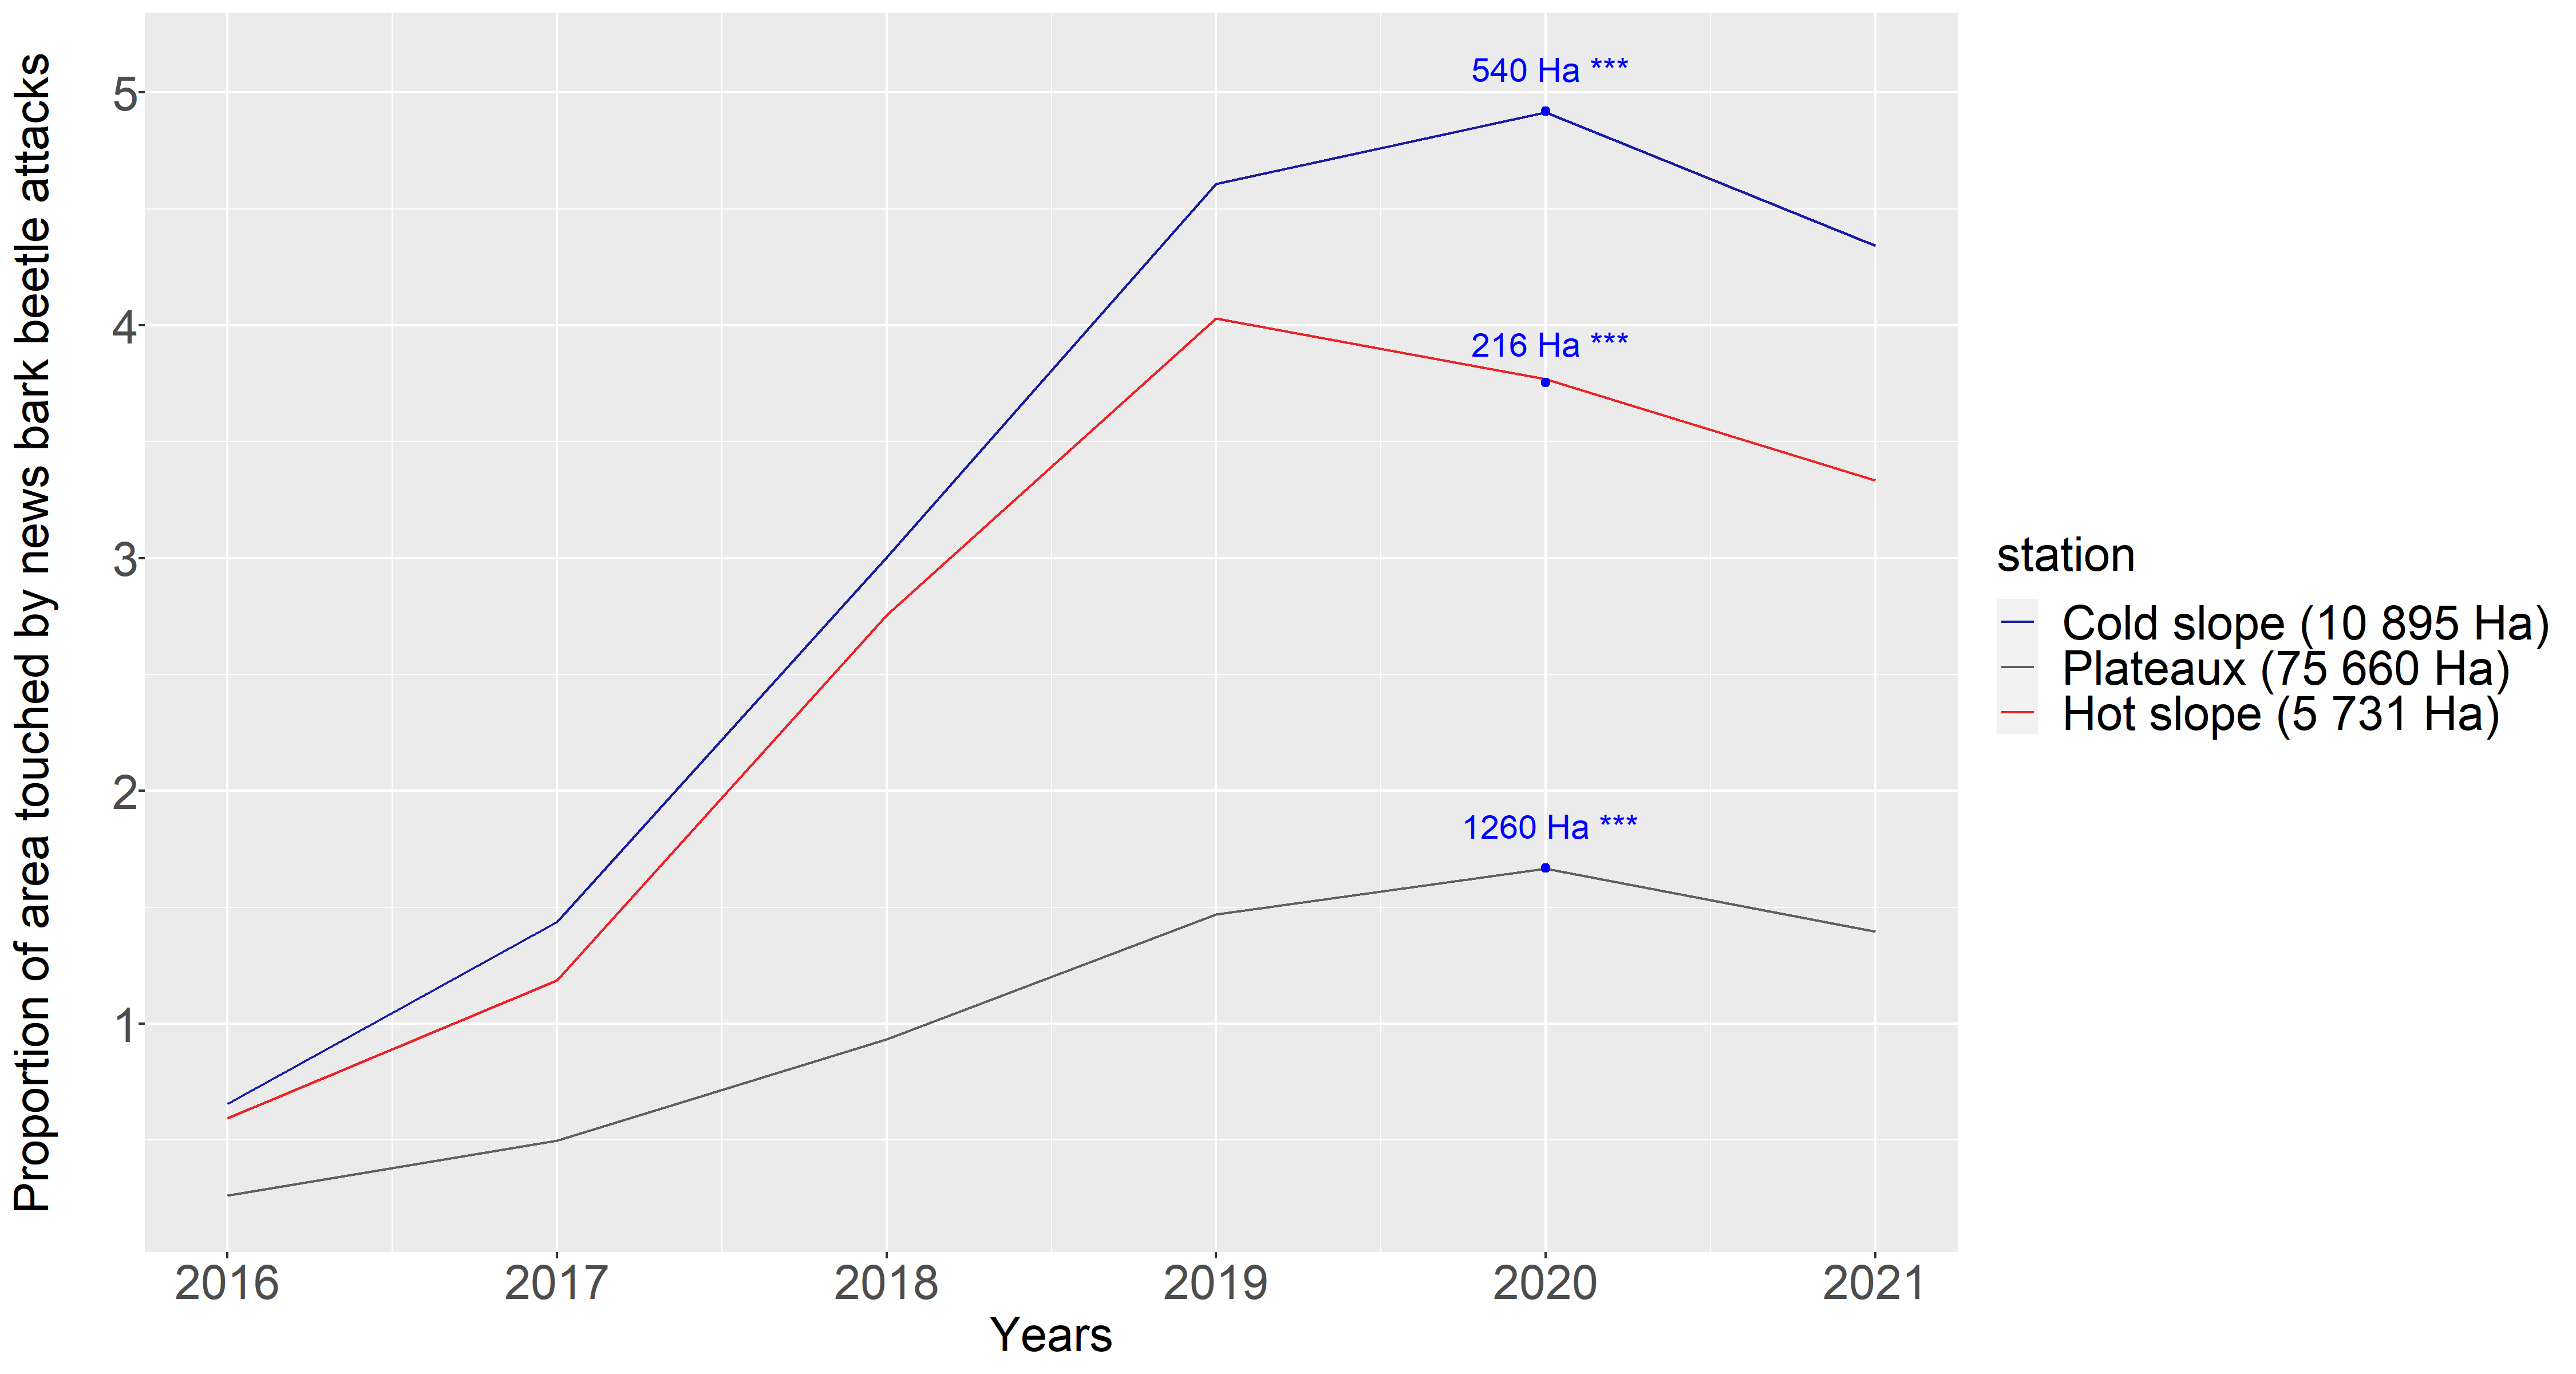
\includegraphics[width=1\textwidth]{evol_ss_wal.png}
%		\caption{Évolution de la crise du typographe en région wallonne en fonction des sous-secteurs.}
%		\label{fig:ss_wall}
		%\caption sert à insérer une légende
%	\end{minipage}\hfill
%	\vspace{1cm}
%	\begin{minipage}[b]{1 \linewidth}
%		\centering
%		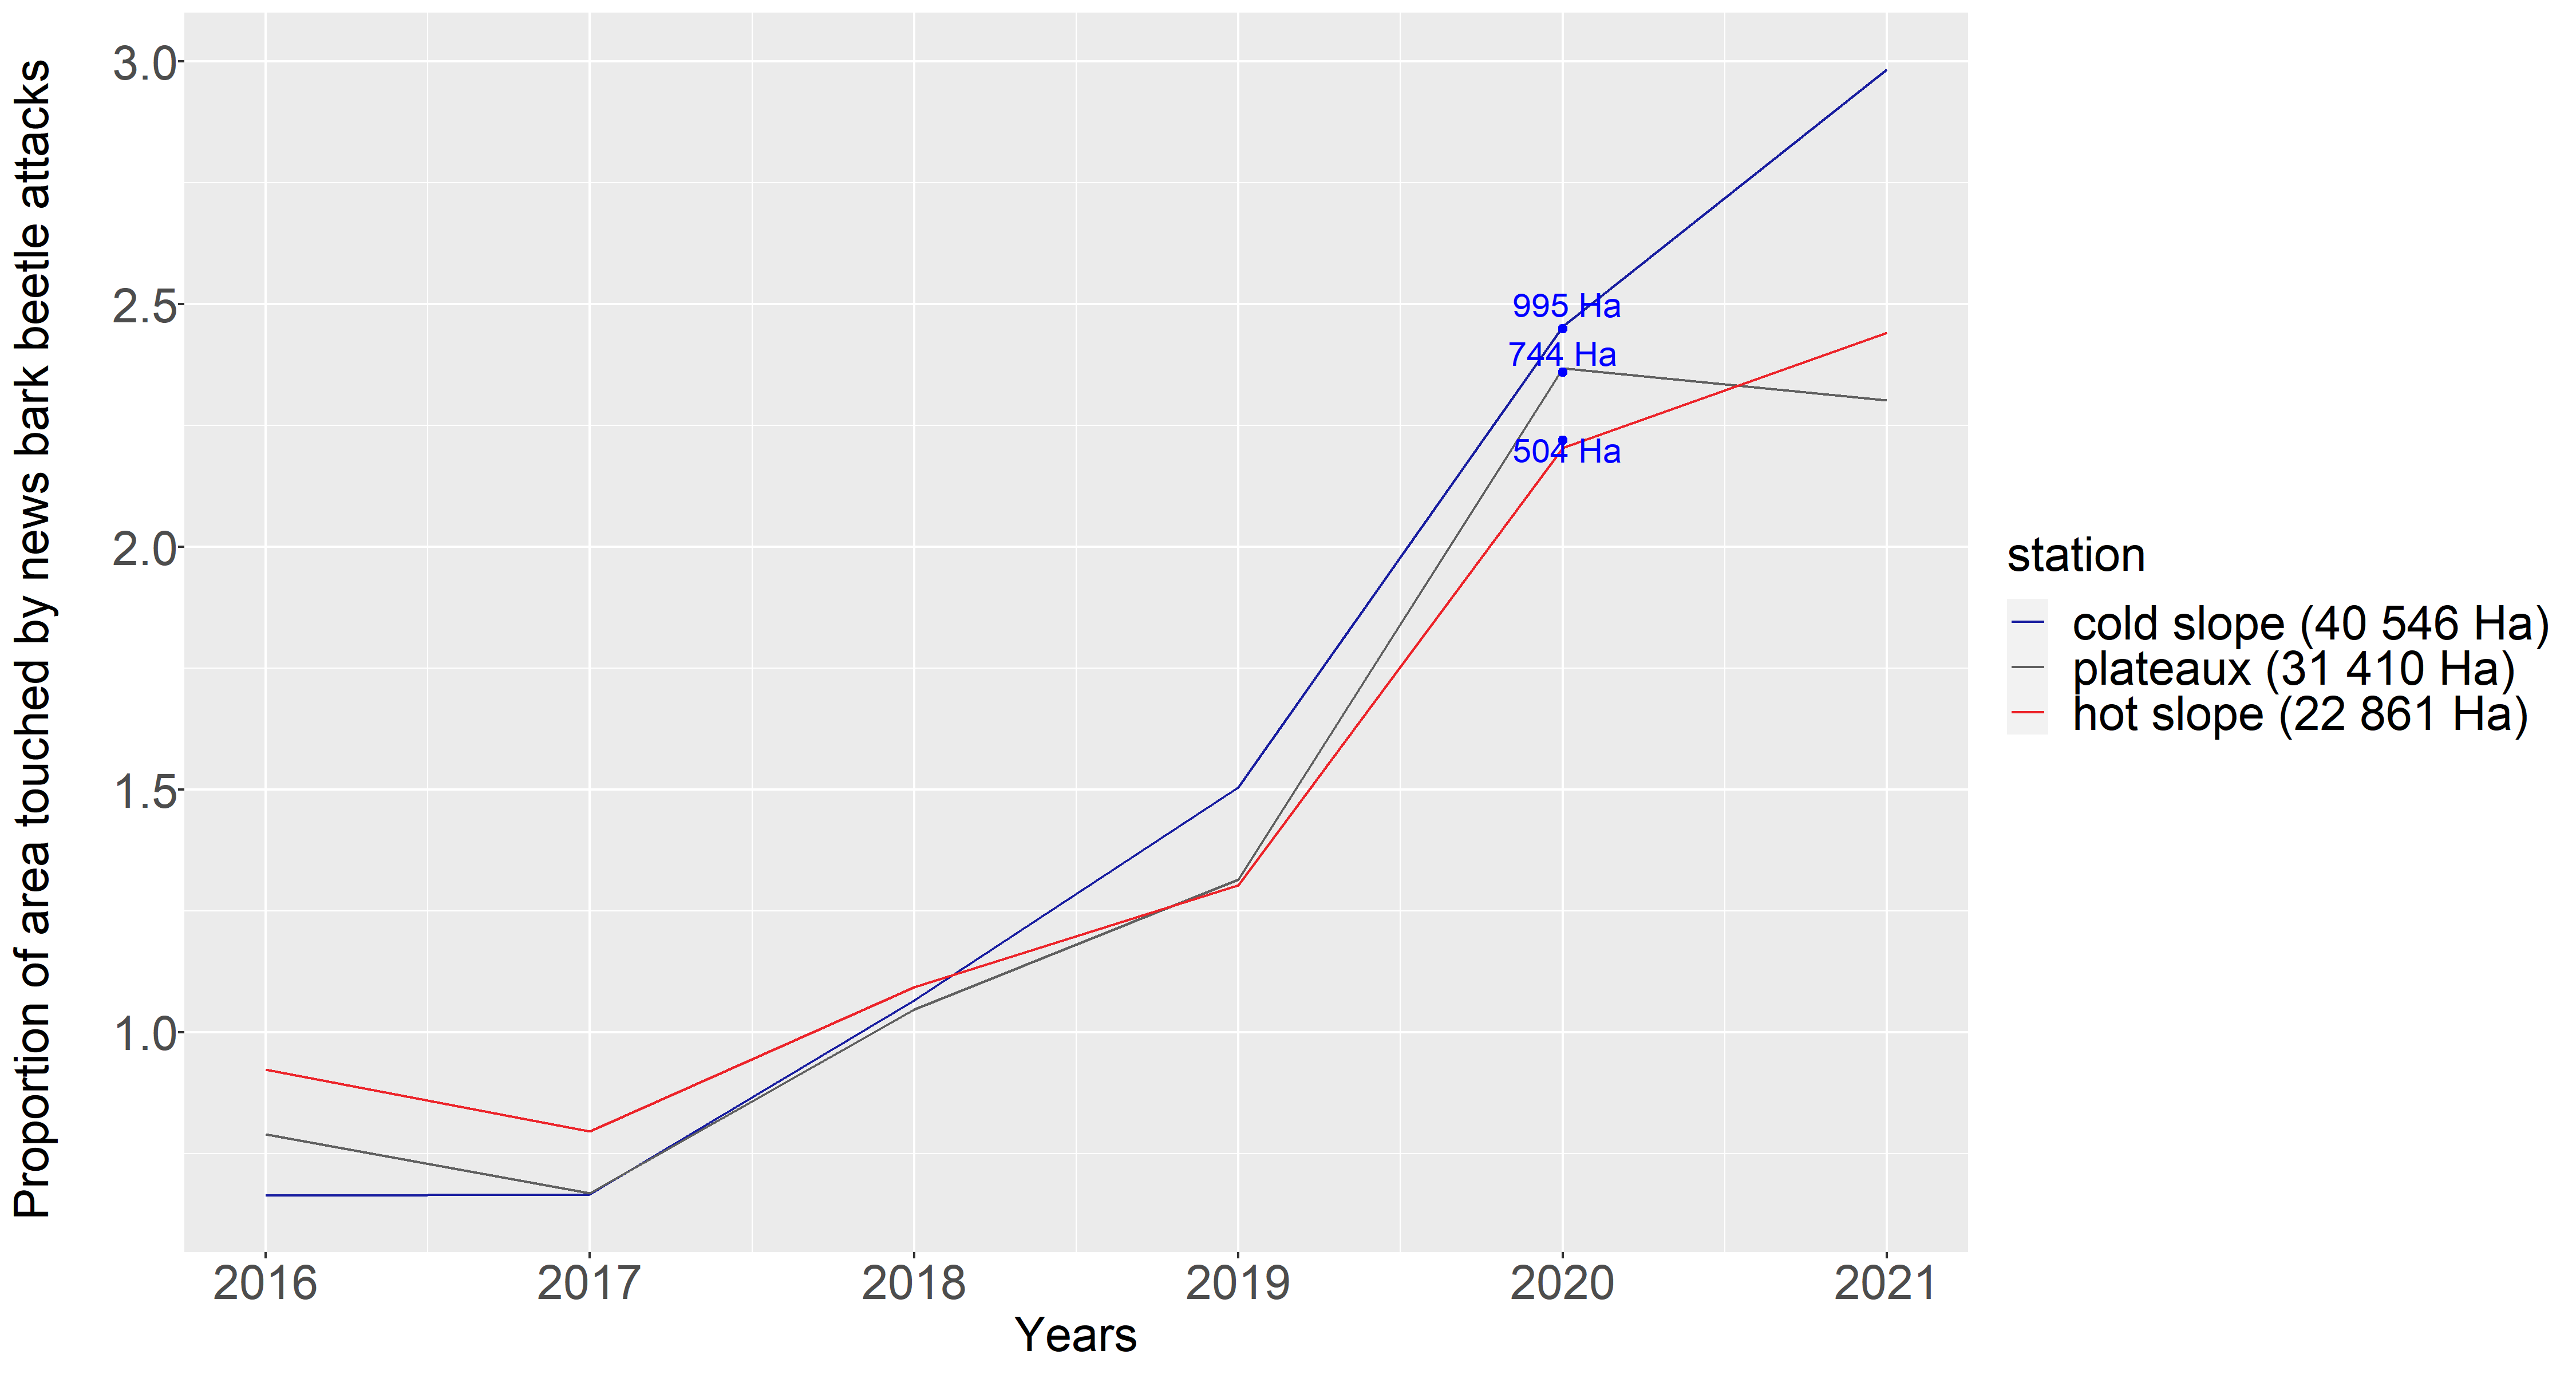
\includegraphics[width=1\textwidth]{evol_ss_vosges.png}
%		\caption{Évolution de la crise du typographe dans les Vosges en fonction des sous-secteurs .}
%		\label{fig:ss_vosg}
%	\end{minipage}
%end{figure}

\section{Acknowledgements}

This research has been funded thanks to the \textit{RegioWood II} project and to the \textit{Plan quinquennal de recherches forestières} of the Service Public de Wallonie (forest administration).

%\bibliographystyle{elsarticle-num}
\bibliographystyle{plainnatGL_v2}\biboptions{authoryear}
\bibliography{Scolyte.bib}
\end{document}